\documentclass[letter,12pt]{article} % This defines the style of your paper
\usepackage{times}

\usepackage[top = 2.5cm, bottom = 2.5cm, left = 2.5cm, right = 2.5cm]{geometry} %margen%

\usepackage[T1]{fontenc}
\usepackage[utf8]{inputenc}

\usepackage{multirow} % Multirow is for tables with multiple rows within one cell.
\usepackage{booktabs} % For even nicer tables.

% As we usually want to include some plots (.pdf files) we need a package for that.
\usepackage{graphicx} 

% The default setting of LaTeX is to indent new paragraphs. This is useful for articles. But not really nice for homework problem sets. The following command sets the indent to 0.
\usepackage{setspace}
\setlength{\parindent}{0in}

% Package to place figures where you want them.
\usepackage{float}

% The fancyhdr package let's us create nice headers.
\usepackage{fancyhdr}

\usepackage{amsmath,mathtools}
\usepackage{epstopdf}
\usepackage{amsfonts}
\usepackage{amssymb}
\usepackage{graphicx}
\usepackage{xcolor}
\usepackage{pdfpages}
\usepackage{epstopdf}

%%%%%%%%%%%%%%%%%%%%%%%%%%%%%%%%%%%%%%%%%%%%%%%%
% 3. Header (and Footer)
%%%%%%%%%%%%%%%%%%%%%%%%%%%%%%%%%%%%%%%%%%%%%%%%

\pagestyle{fancy} % With this command we can customize the header style.

\fancyhf{} % This makes sure we do not have other information in our header or footer.

\lhead{\footnotesize BD01-2022-1: Proyecto Final}% \lhead puts text in the top left corner. \footnotesize sets our font to a smaller size.

%\rhead works just like \lhead (you can also use \chead)
\rhead{\footnotesize Jimenez, Mora, Resendiz, Valdelamar} %<---- Fill in your lastnames.

% Similar commands work for the footer (\lfoot, \cfoot and \rfoot).
% We want to put our page number in the center.
\cfoot{\footnotesize \thepage} 


%%%%%%%%%%%%%%%%%%%%%%%%%%%%%%%%%%%%%%%%%%%%%%%%
% 4. Your document
%%%%%%%%%%%%%%%%%%%%%%%%%%%%%%%%%%%%%%%%%%%%%%%%

\begin{document}%inicio del docu%
\thispagestyle{empty} % This command disables the header on the first page. 
{\small
\begin{tabular}{
 p{0.78\textwidth}  p{0.22\textwidth}}% This is a simple tabular environment to align your text nicely 
	
\includegraphics[scale=0.55]{imagenes/UNAM.png} & 
\includegraphics[scale=0.43]{imagenes/UNAMFI.png}


%\hline % \hline produces horizontal lines.
\end{tabular} % Our tabular environment ends here.
}


% Datos caratula
\begin{center} 
\Huge{Universidad Nacional Aut\'onoma de M\'exico
}
\par\vspace{1.5cm}
{
\Huge{  Facultad de Ingenier\'ia
}
}
\par\vspace{1cm}
{
\large{  Asignatura: \textbf{Bases de Datos}
}
}
\par\vspace{0.5cm}
{
\large{  Profesor:  \textbf{Ing. Fernando Arreola Franco}
}
}
\par\vspace{0.5cm}
{
\large{ \textbf{ Proyecto Final}
}
}
\par\vspace{0.5cm}
{
\large{ Equipo: \textbf{RAJAVX}
}
}
\par\vspace{0.5cm}
{
\large{ Alumnos: 
\\ \textbf{Jimenez Avila Javier Alejandro
\\Mora Castro Fernando Alexis
\\Resendiz Cruz Rodrigo Daniel
\\Valdelamar Tamez Valeria
}\\
}
}
\par\vspace{0.5cm}
{
\large{ Grupo:  \textbf{1°}
}
}
\par\vspace{0.5cm}
{
\large{ Semestre:  \textbf{2022-1}
}
}
\par\vspace{0.5cm}
{
\large{ Fecha:  \textbf{11 de Diciembre 2021}
}
}
		
\end{center}  

\vspace{0.4cm}

%%%%%%%%%%%%%%%%%%%%%%%%%%%%%%%%%%%%%%%%%%%%%%%%



\newpage
\large{ \textbf{Introducci\'on}}
\\\\
Planteamiento
\\\\
Este proyecto tiene el fin de realizar una base de datos para la administración de una cadena de papelerías, que tenga almacenado los datos de los proveedores tales cómo;  la razón social, domicilio, nombre y teléfonos de los proveedores, rfc, nombre, domicilio y al menos un email de los clientes,  el inventario de productos en venta en el que debe guardarse; el código de barras, precio al que fue comprado el producto, fecha de compra y cantidad de ejemplares en la bodega (stock, existencias), los datos que se desean guardar de los diferentes artículos son; la marca, descripción y precio de los regalos, artículos de papelería, impresiones y
recargas, siempre y cuando se tenga su correspondiente registro en el inventario, de las ventas; el número de venta, fecha de venta y la cantidad total a pagar de la venta, así como la cantidad de cada artículo y precio total a pagar por artículo.
\\\\
Además que:
\begin{itemize}
\item Al recibir el código de barras de un producto, regrese la utilidad.
\item Cada que haya la venta de un artículo, deberá decrementarse el stock por la cantidad vendida de ese artículo. Si el valor llega a cero, abortar la transacción. Si el pedido se completa pero quedan menos de 3 en stock, se deberá emitir una alerta.
\item Dada una fecha, o una fecha de inicio y fecha de fin, regresar la cantidad total que se vendió y la ganancia correspondiente en esa fecha/periodo.
\item Permitir obtener el nombre de aquellos productos de los cuales hay menos de 3 en stock.
\item Generar de forma automática la factura de una compra.
\item Realizar los índices que se requieran.\\
\end{itemize}
Deberán tomarse las siguientes consideraciones:
\begin{itemize}
\item El número de venta debe tener un formato similar a "VENT-001".
\item Donde esté presente el atributo domicilio, este debe estar compuesto por estado, código postal, colonia, calle y número. \newpage
\end{itemize}
Objetivos
\begin{enumerate}
\item Aplicar los conceptos y técnicas vistas en clase para diseñar y crear una base de datos y su administración para una cadena de papelerías, que cumpla con las características propias del solicitante.
\item Hacer buen uso del tiempo para poder desarrollar y solucionar nuestra problemática.
\\\\
\end{enumerate}
Propuesta de Resolución
\\\\
Fue enumerada en una serie de 11 pasos a seguir:
\begin{enumerate}
\item Empezar con el diseño de nuestra base de datos, en primera instancia la lectura y comprensión de lo que se nos pide.
\item Organizar la participación del equipo de trabajo así cómo la asignación de tareas que le tocará a cada integrante.
\item La puntualización de reuniones necesarias para ir revisando el avance del proyecto. 
\item Realizar el diagrama entidad relación de nuestra base de datos,y después el diagrama relacional.
\item La creación de la base de datos y sus tablas (campos, relaciones y restricciones) en el manejador.
\item Programación SQL sobre los requerimientos dados.
\item Diseño y Programación de la interfaz gráfica.
\item Conexión de nuestra base de datos con la interfaz gráfica, y pruebas de su funcionamiento.
\item Elaboración de la documentación y manual de usuario.
\item Pruebas finales de nuestra base de datos y de su adecuado funcionamiento.
\item Preparación de la exposición del proyecto.
\end{enumerate}
\newpage
\large{ \textbf{Plan de Trabajo}}
\\\\
Se decidió organizar todas nuestras actividades por medio de un diagrama de Gantt:
\begin{center} 
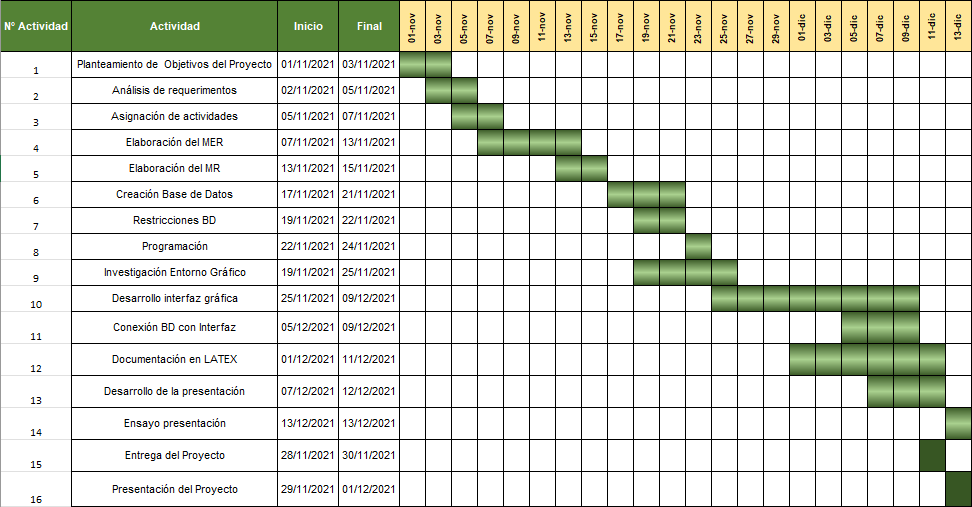
\includegraphics[scale=0.64]{imagenes/DGANTT.png}
\end{center}
La organización de actividades por parte del equipo fue la siguiente:
\begin{center} 
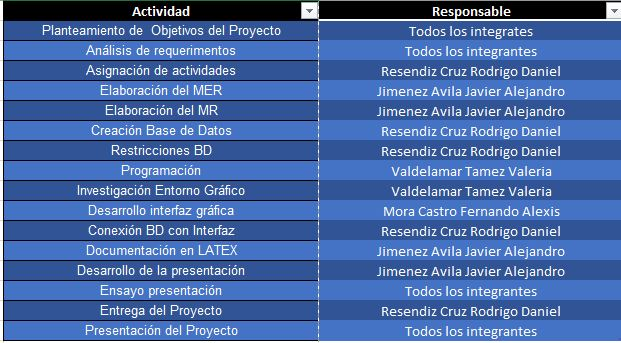
\includegraphics[scale=0.95]{imagenes/DA.JPG}
\end{center}
\newpage
\large{ \textbf{Diseño}}
\\\\
Realizamos el primer bosquejo de la base de datos, posteriormente se realizó la afinación del diseño y estructura de esta misma por medio del diagrama entidad relación.
\\\\
Modelo Entidad Relaci\'on:
\\\\
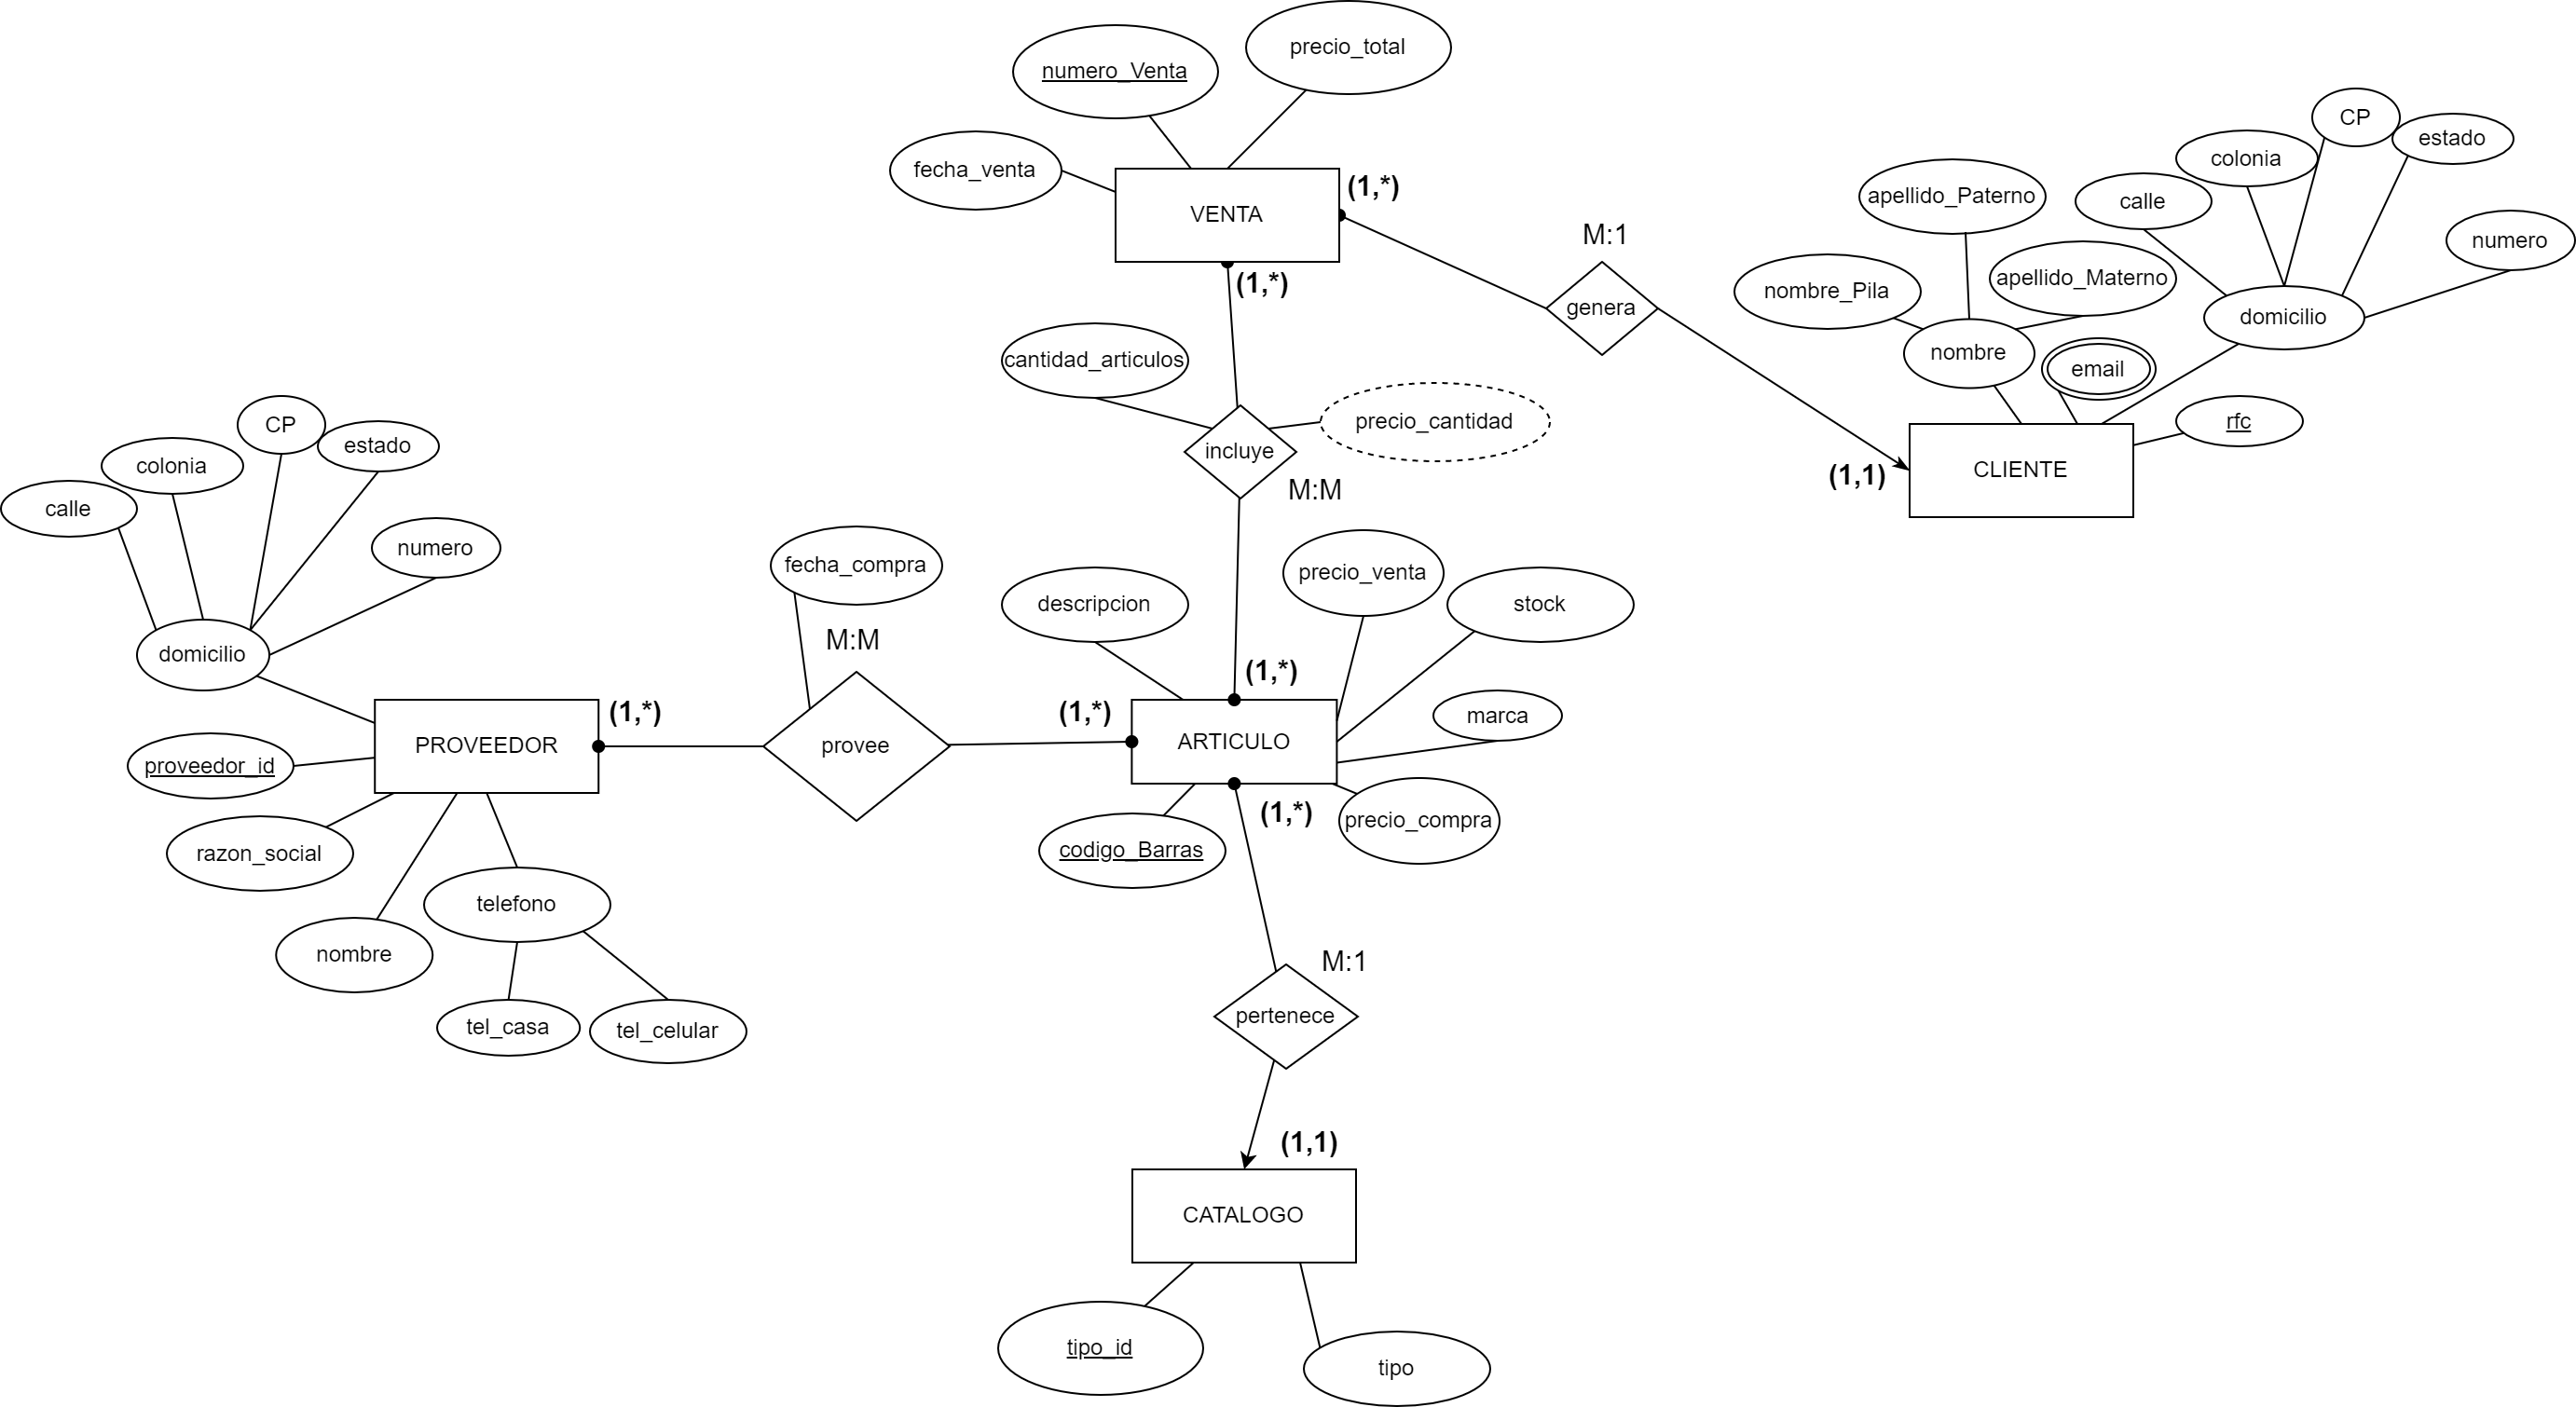
\includegraphics[scale=0.17]{imagenes/MER.png}
\\\\
Descripción:
\\\\
Nuestro Modelo Entidad Relación fue hecho con base a los requerimientos dados. Empezaremos explicando la tabla Proveedor que es una subtabla de la tabla artículo, esta tabla guardará los datos del proveedor, consta de 5 atributos principales; domicilio (que se descompone en un subtabla con los atributos; calle, colonia, cp, estado y número), proveedor\_id, razón\_social, nombre y teléfono (siendo una subtabla con los campos tel\_casa y tel\_celular), en el caso del atributo teléfono elegimos que fuera también una tabla, para evitar que fuera multivaluado, lo cual se pensó de forma estratégica, ya que no lo vimos necesario. Su cardinalidad según lo analizado es de 1:M en relación con la tabla del artículo.
\\\\
Después tenemos la tabla artículo que está compuesta de 6 atributos, los cuales son; descripción, precio\_venta, stock (existencias), marca, precio\_compra y código\_barras. El precio de venta es a lo que la papelería venderá el artículo y el precio\_compra es a lo que lo compró la papelería. Esta tabla está unida con tres tablas (subtablas); una llamada venta con cardinalidad 1:M, después con dos tablas subyacentes; la de proveedor que ya la mencionamos con anterioridad, con cardinalidad 1:M,  y la tabla catálogo, con cardinalidad 1:1 que explicaremos a continuación:
\\\\
La tabla catálogo alberga los tipos de productos que existirán en el almacén, cuenta con solo dos atributos; tipo\_id y tipo, el número y nombre del artículo.
\\\\
La tabla venta, subtabla de artículo y de la tabla cliente, esta tabla tiene el fin de guardar el número de artículos comprados, su precio unitario, el precio total  y la fecha de la compra, tiene 5 atributos puntualizando, los cuales son; fecha\_venta, numero\_venta, precio\_total, cantidad\_articulos y precio\_cantidad. En la relación venta-articulos tiene una cardinalidad de 1:M y la relación con la tabla cliente su cardinalidad es de 1:M – M:1 y de 1:1. 
\\\\\\
Normalización
\begin{itemize}
\item Primera Forma normal: sí cumple, ya que no presenta grupos de repetición y cada columna contienen valores atómicos.
\item Segunda Forma Normal: De terminaremos si existen relaciones parciales con base al diagrama relacional:
\begin{center} 
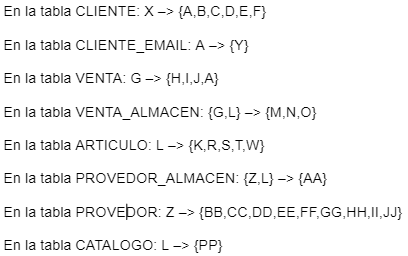
\includegraphics{imagenes/N.png}
\end{center}
\item Tercera Forma Normal: Sí cumple ya que se encuentra en 2FN y cualquier atributo no -principal de la tabla no es transitivamente dependiente de cada clave candidata de la misma. \\\\\\
\end{itemize}
Modelo Relacional:
\\
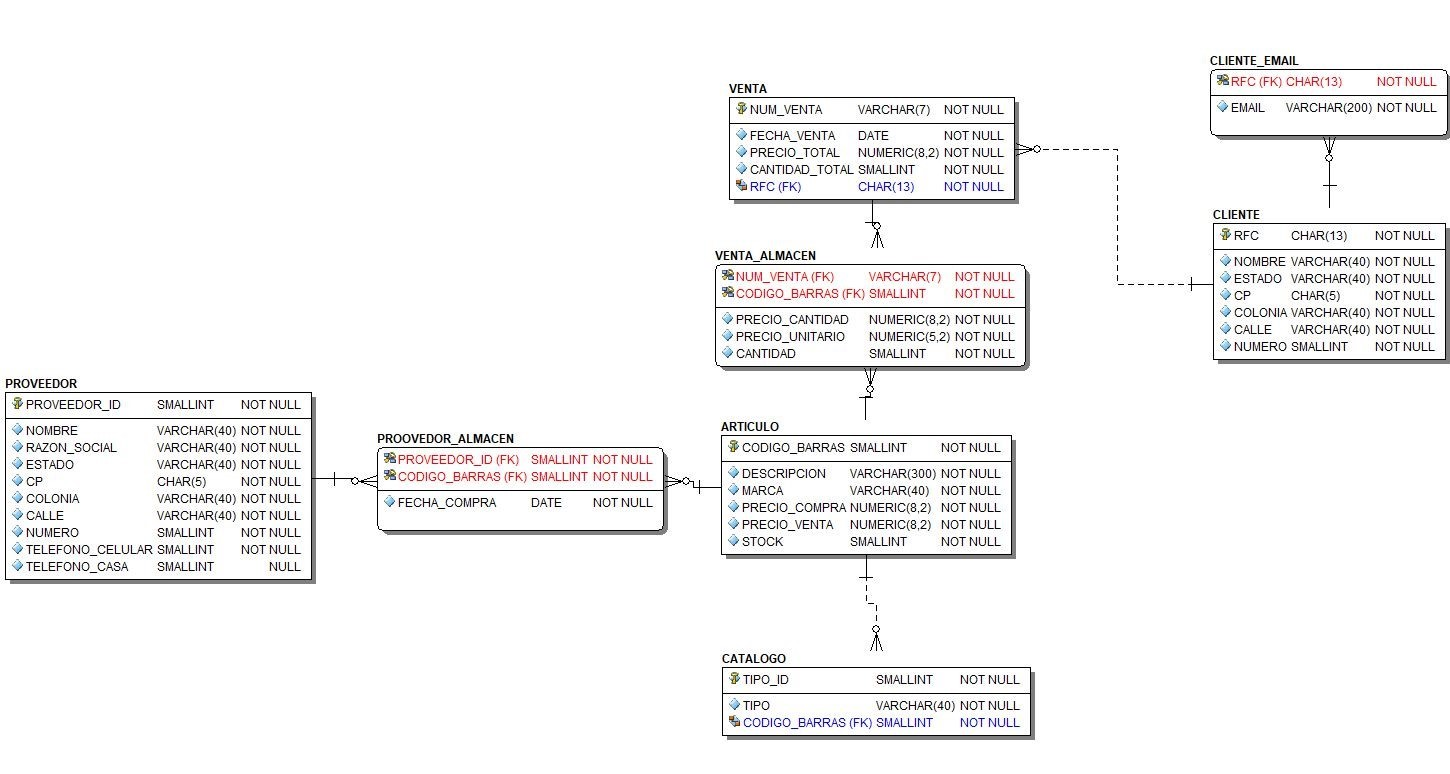
\includegraphics[scale=0.43]{imagenes/MR01.jpg}
\\
Descripción:
\\\\
Para el modelo relacional se agregaron las tablas “proveedor\_almacen” y la tabla “venta\_almacen” las cuales van a guardar un registro detallado de las ventas que se efectúen y de las compras de los productos. Adicionalmente se creó una tabla llamada “cliente\_email” el cual se encargará de almacenar los email de los clientes, en esa tabla.
\newpage
Modelo Lógico:
\\
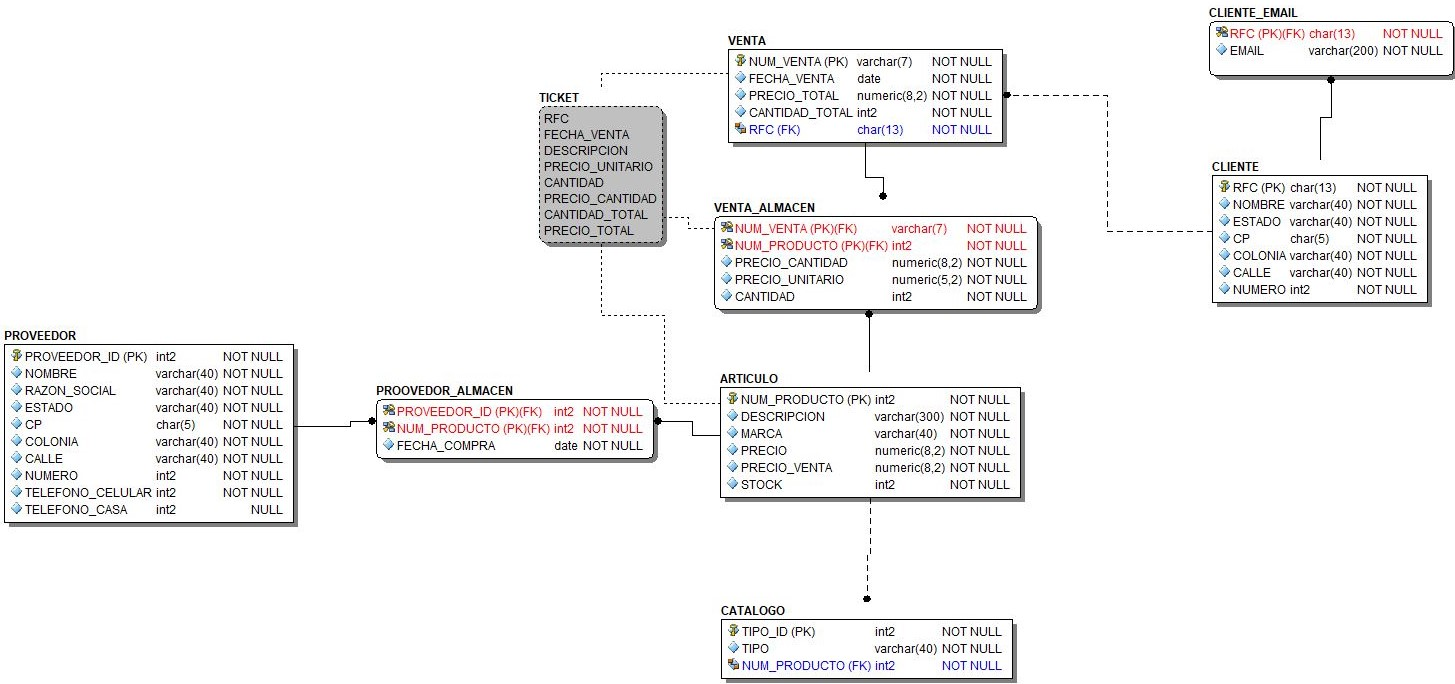
\includegraphics[scale=0.43]{imagenes/MR02.jpg}
\\
Descripción:
\\\\
En el modelo lógico se tiene lo mismo que en el modelo relacional, pero, se agrega la vista llamada como ticket que se nos solicita generar mediante el registro de las ventas.
\\\\\\
\large{ \textbf{Implementaci\'on}}
\\\\
Funcionamiento los bloques de programación:
\\\\
\begin{center} 
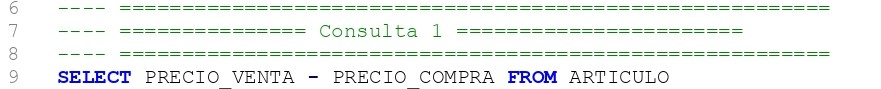
\includegraphics{imagenes/B01.jpg}
\end{center}
Explicación: Se toma de cada artículo el precio de compra y el precio de venta, estos dos se restan y la consulta regresa el resultado de esta operación matemática, siendo esta la utilidad de cada artículo.
\newpage
\begin{center} 
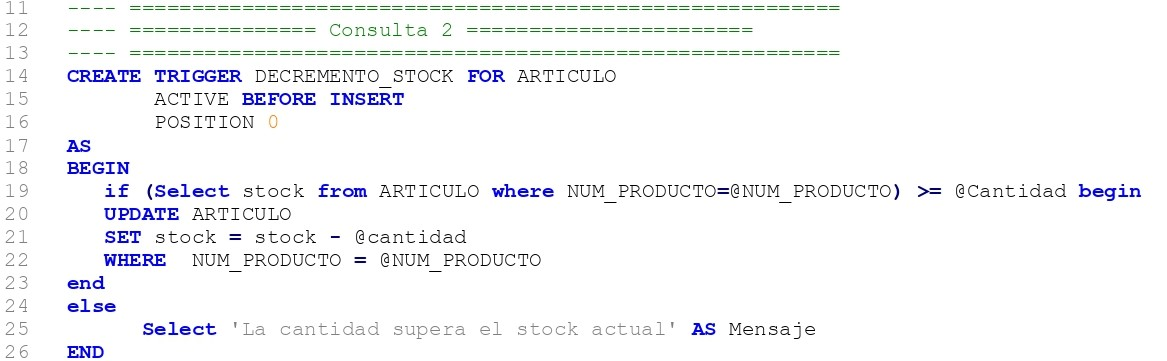
\includegraphics[scale=0.85]{imagenes/B02.jpg}
\end{center}
Explicación: Se crea un trigger que se dispara antes del insert cuando esté se dispara se buscará el stock del artículo en cuestión mediante su número de producto, si este stock es mayor a la cantidad 0 se actualizará el stock de el producto encontrado, el stock actualizado será stock menos cantidad, de lo contrario si el stock es menor a 0 se regresa una alerta.
\\\\\\
\begin{center} 
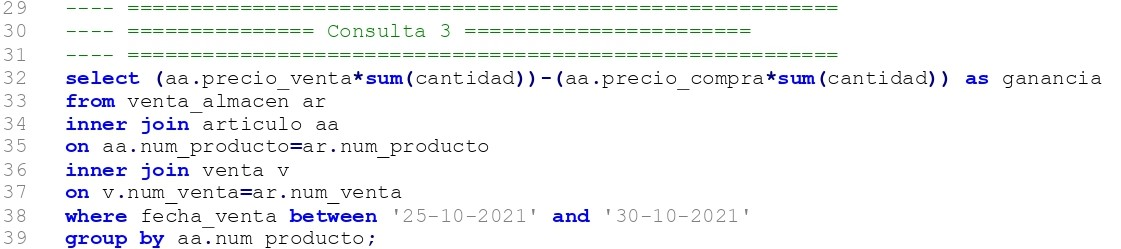
\includegraphics[scale=0.85]{imagenes/B03.jpg}
\end{center}
Explicación: De la venta del almacén se obtiene su ganancia, precio venta por cantidad menos precio compra por cantidad, teniendo la ganancia se busca el artículo de esta respectiva ganancia mediante un join usando el número de producto, ahora bien se realiza un segundo join para encontrar la fecha de la venta, este segundo join se realiza mediante el número de venta; finalmente los resultados se agrupan mediante el número de producto.
\newpage
\begin{center} 
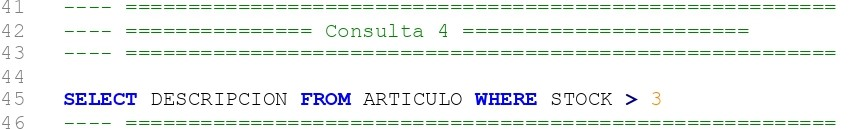
\includegraphics{imagenes/B04.jpg}
\end{center}
Explicación: Se busca la descripción de los artículos donde su stock es mayor a 3.
\\\\\\
\begin{center} 
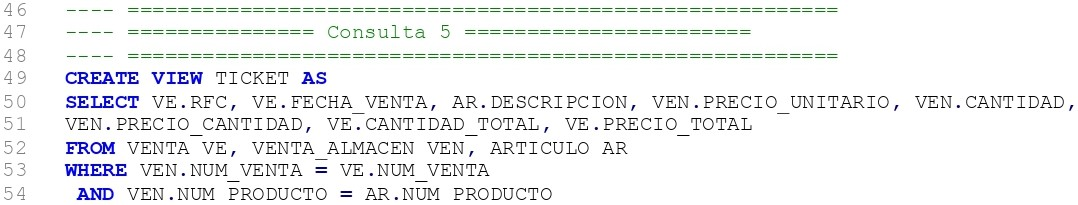
\includegraphics[scale=0.85]{imagenes/B05.jpg}
\end{center}
Explicación: Se crea una vista llamada ticket que busca rfc, fecha de venta, descripción, precio unitario, cantidad, precio cantidad, cantidad total y precio total de las tablas venta, venta almacén y artículo usando el número de venta y número de producto como filtros; esta información obtenida es usada para la generación de facturas.\\
La generación de la vista nos permite realizar consultas más complejas sobre esta información ya que genera una tabla virtual, por el contrario de estar consultando toda la información mediante selects. 
\newpage
DDL:
\\\\
El ddl contiene la definición de las tablas para ser implementadas dentro de la base de datos, la creación de las tablas se muestra a continuación:
\\\\
Tabla producto:
\begin{center} 
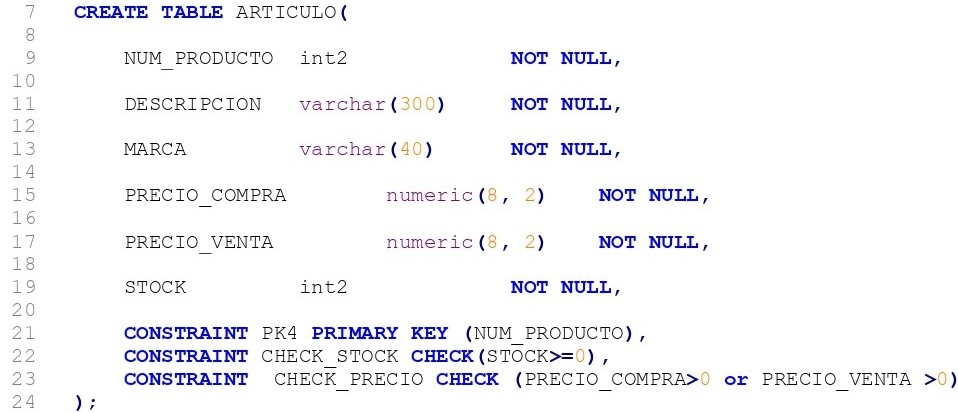
\includegraphics[scale=0.90]{imagenes/DDL01.jpg}
\end{center}
En la tabla producto se tiene la definición de las columnas que se van a emplear y se agregan como constraints la llave primaria la cual es el número de producto, un check que verifica que el precio de compra sea mayor que 0 y el stock sea mayor o igual a 0, se permite que el stock sea igual a cero porque pueden acabarse los artículos en la papelería, pero siguen estando en el catálogo de productos.
\\\\\\
Tabla Catalogo:
\begin{center} 
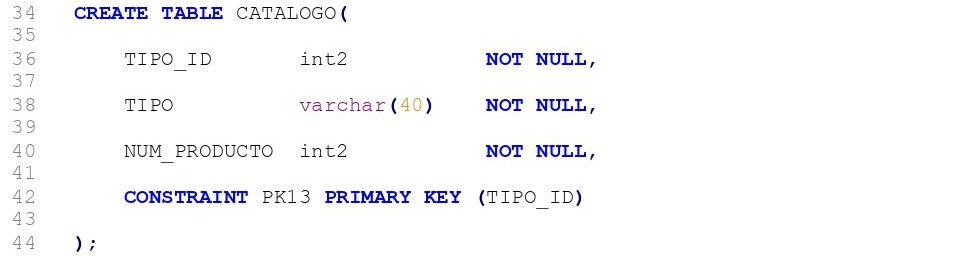
\includegraphics[scale=0.90]{imagenes/DDL02.jpg}
\end{center}
En la tabla catálogo se añadió el identificador para cada tipo de artículo con respecto a cada  producto registrado. 
\newpage
Tabla Cliente:
\begin{center} 
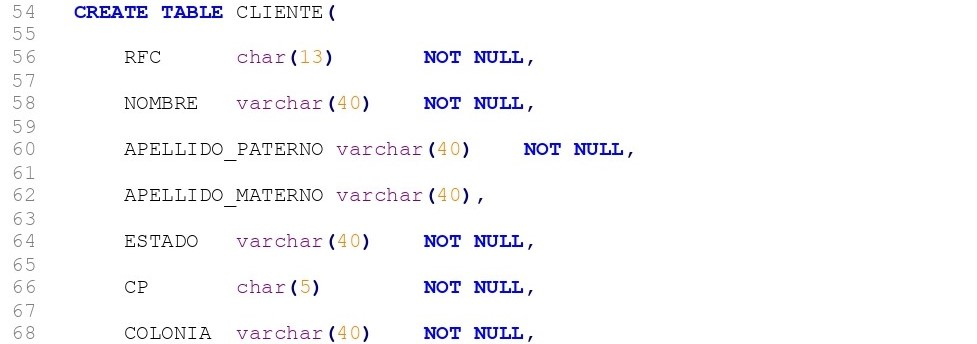
\includegraphics[scale=0.90]{imagenes/DDL03-1.jpg}
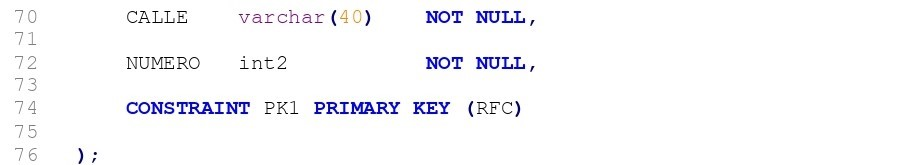
\includegraphics[scale=0.90]{imagenes/DDL03-2.jpg}
\end{center}
En la tabla cliente se definen los campos del nombre completo desglosado y los datos del domicilio del cliente. El RFC del cliente tiene que ser de 13 caracteres.
\\\\\\
Tabla Cliente\_Email:
\begin{center} 
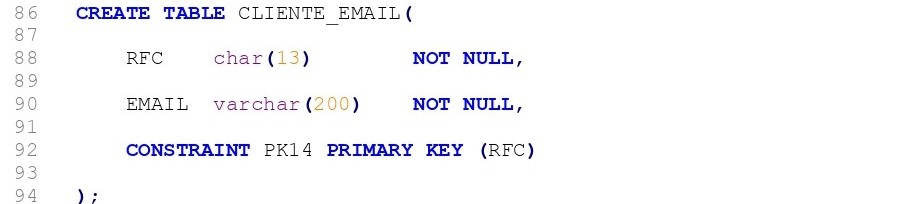
\includegraphics[scale=0.90]{imagenes/DDL04.jpg}
\end{center}
La tabla cliente\_email es la que se encarga de almacenar los correos de cada cliente, este toma como parámetros el RFC del cliente y su email.
\newpage
Tabla proveedor\_almacen:
\begin{center} 
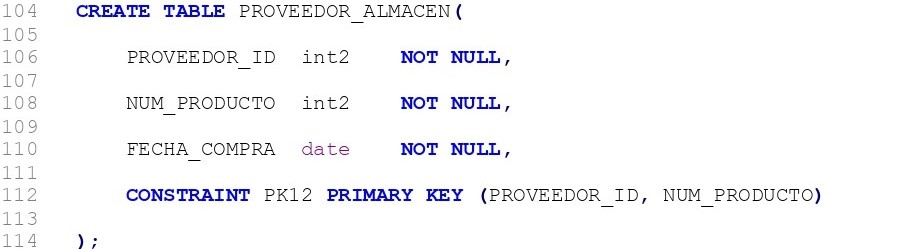
\includegraphics[scale=0.90]{imagenes/DDL05.jpg}
\end{center}
En la tabla proveedor almacén se tienen los datos asociados a la compra de los artículos con una llave primaria compuesta de el id del proveedor al que se le compró junto con el artículo comprado, como columna que no es llave primaria se tiene la fecha de compra de dicho producto a tal proveedor.
\\\\\\
Tabla Proveedor:
\begin{center} 
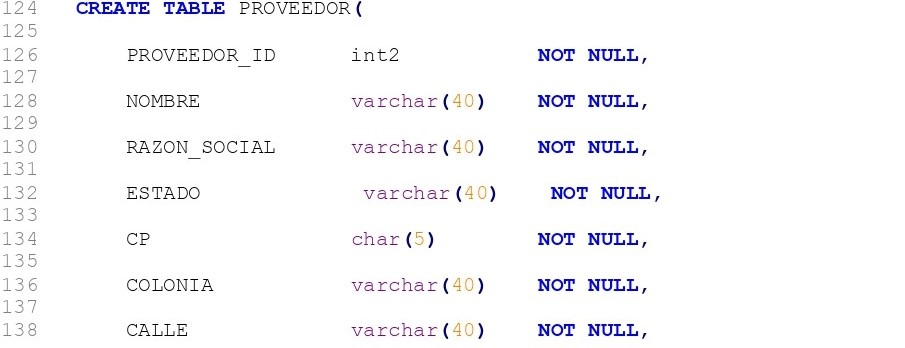
\includegraphics[scale=0.90]{imagenes/DDL06-1.jpg}
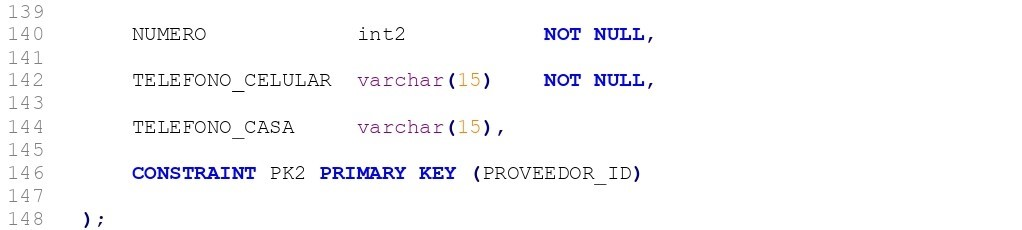
\includegraphics[scale=0.90]{imagenes/DDL06-2.jpg}
\end{center}
La tabla de proveedor es similar al del cliente, solo que se añaden los campos de razón social y los teléfonos asociados a dicho proveedor.
\newpage
Tabla Venta
\begin{center} 
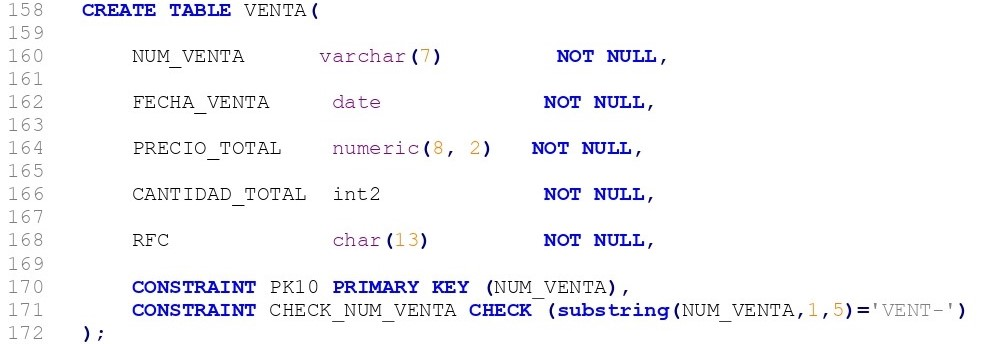
\includegraphics[scale=0.90]{imagenes/DDL07.jpg}
\end{center}
En la tabla venta se tienen los atributos de el número de la venta, la fecha de la venta, el precio total, la cantidad total y el rfc del cliente que hace la compra.
Nótese que se agregó un constraint de tipo check que revisa si el formato de la venta es similar a “VENT-001”.
\\\\\\
Tabla venta almacen:
\begin{center} 
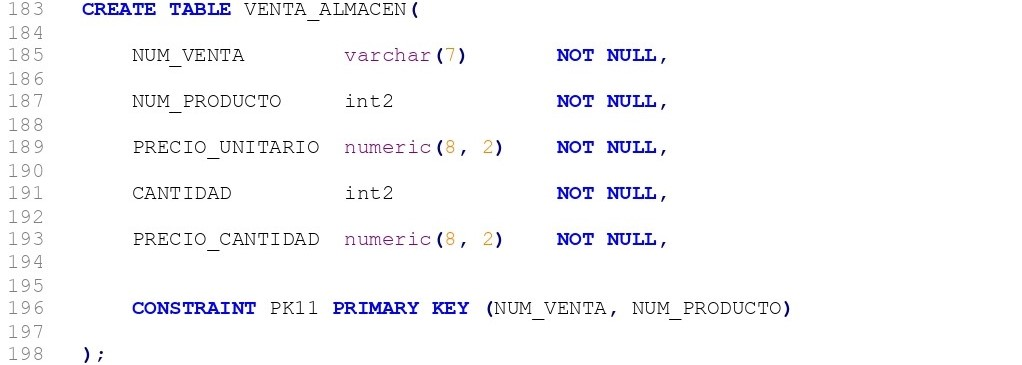
\includegraphics[scale=0.90]{imagenes/DDL08.jpg}
\end{center}
En la tabla venta almacén se agregaron los campos necesarios para registrar de manera más detallada el contenido de los artículos involucrados en una venta. La llave primaria de esta tabla es compuesta ya que se necesitan de los campos del número de venta y el número de producto para conocer el precio del producto involucrado, su cantidad  y su precio de acuerdo a esa cantidad. 
\newpage
Llaves foráneas:
\begin{center} 
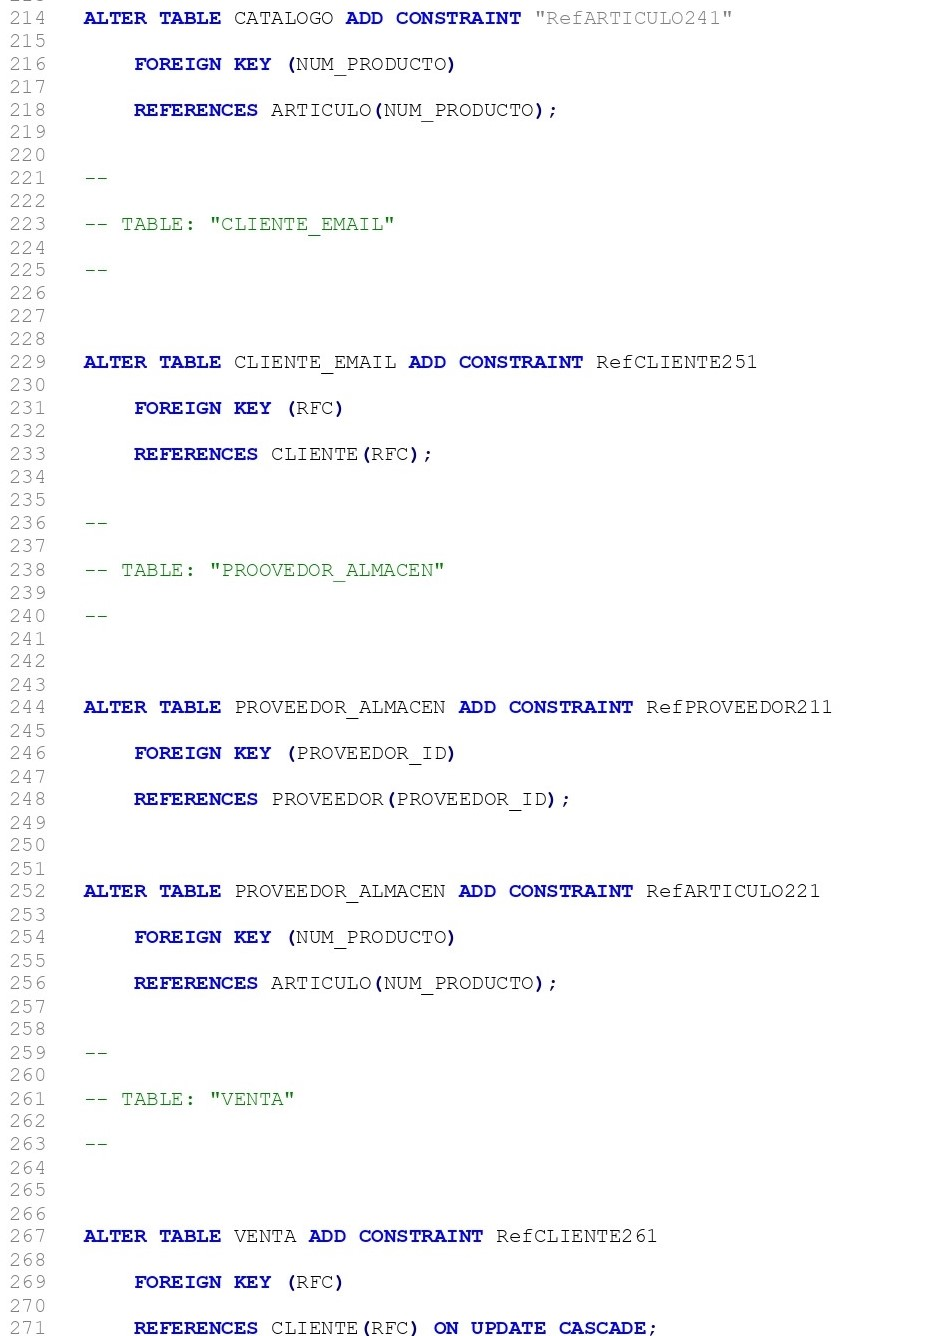
\includegraphics[scale=0.90]{imagenes/DDL09.jpg}
\end{center}
\begin{center} 
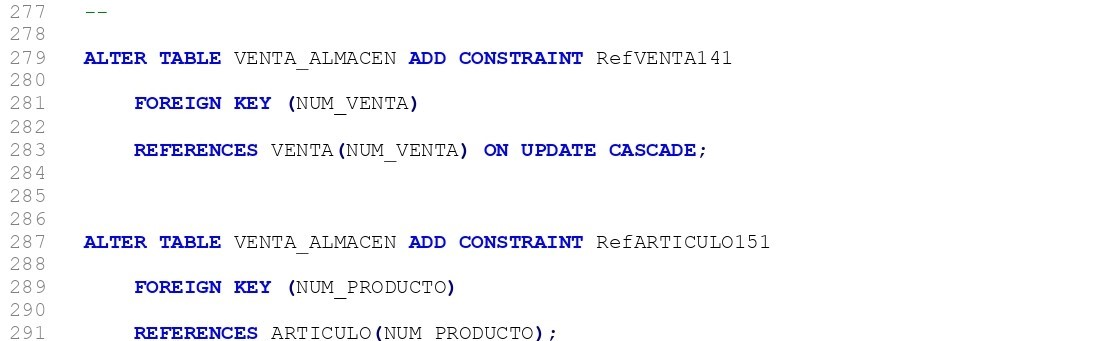
\includegraphics[scale=0.90]{imagenes/DDL10.jpg}
\end{center}
Una vez hechas las tablas se crearon los constraints de llaves foráneas que las enlazan. 
\\\\\\
Secuencia venta:
\begin{center} 
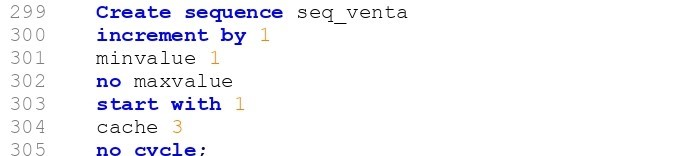
\includegraphics[scale=0.90]{imagenes/DDL11.jpg}
\end{center}
La secuencia venta es una secuencia que se utiliza para obtener el número que va después de “VENT-” la secuencia inicia en 1, su valor mínimo es 1, no tienen valor máximo, inicia en 1 con tres valores en caché y es una secuencia no cíclica.
\\\\\\
Indice nombres empleados:
\begin{center} 
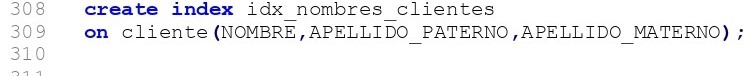
\includegraphics[scale=0.90]{imagenes/DDL12.jpg}
\end{center}

\newpage
El modelo DDL completo se muestra a continuación:
\\\\
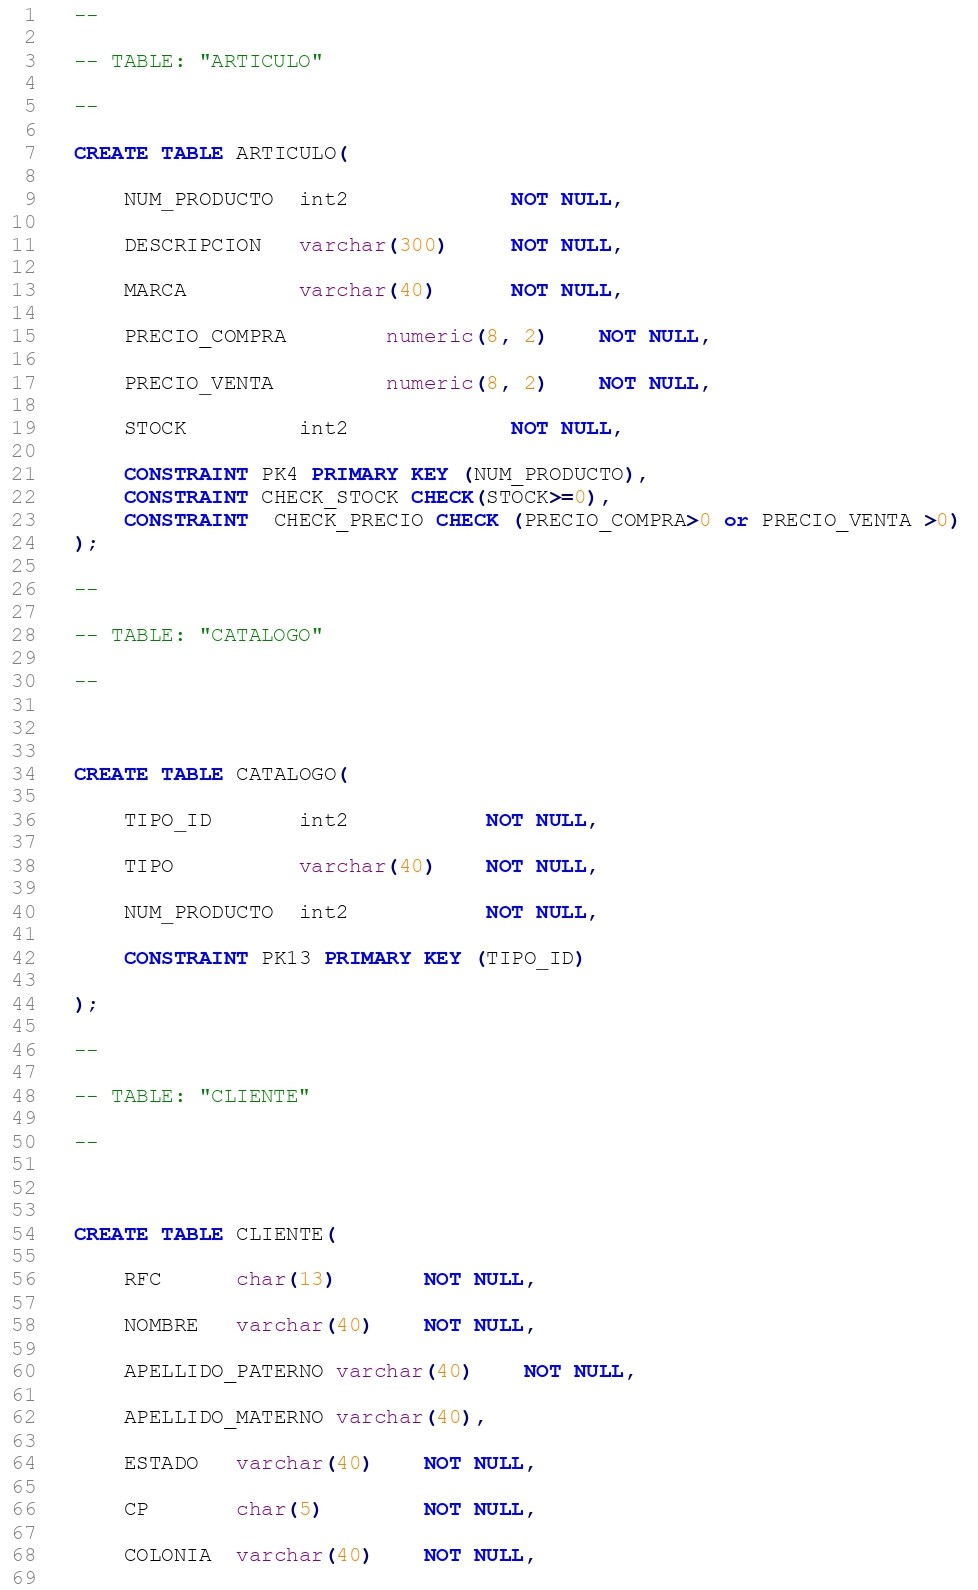
\includegraphics[scale=0.81]{imagenes/DDL1.jpg}
\newpage
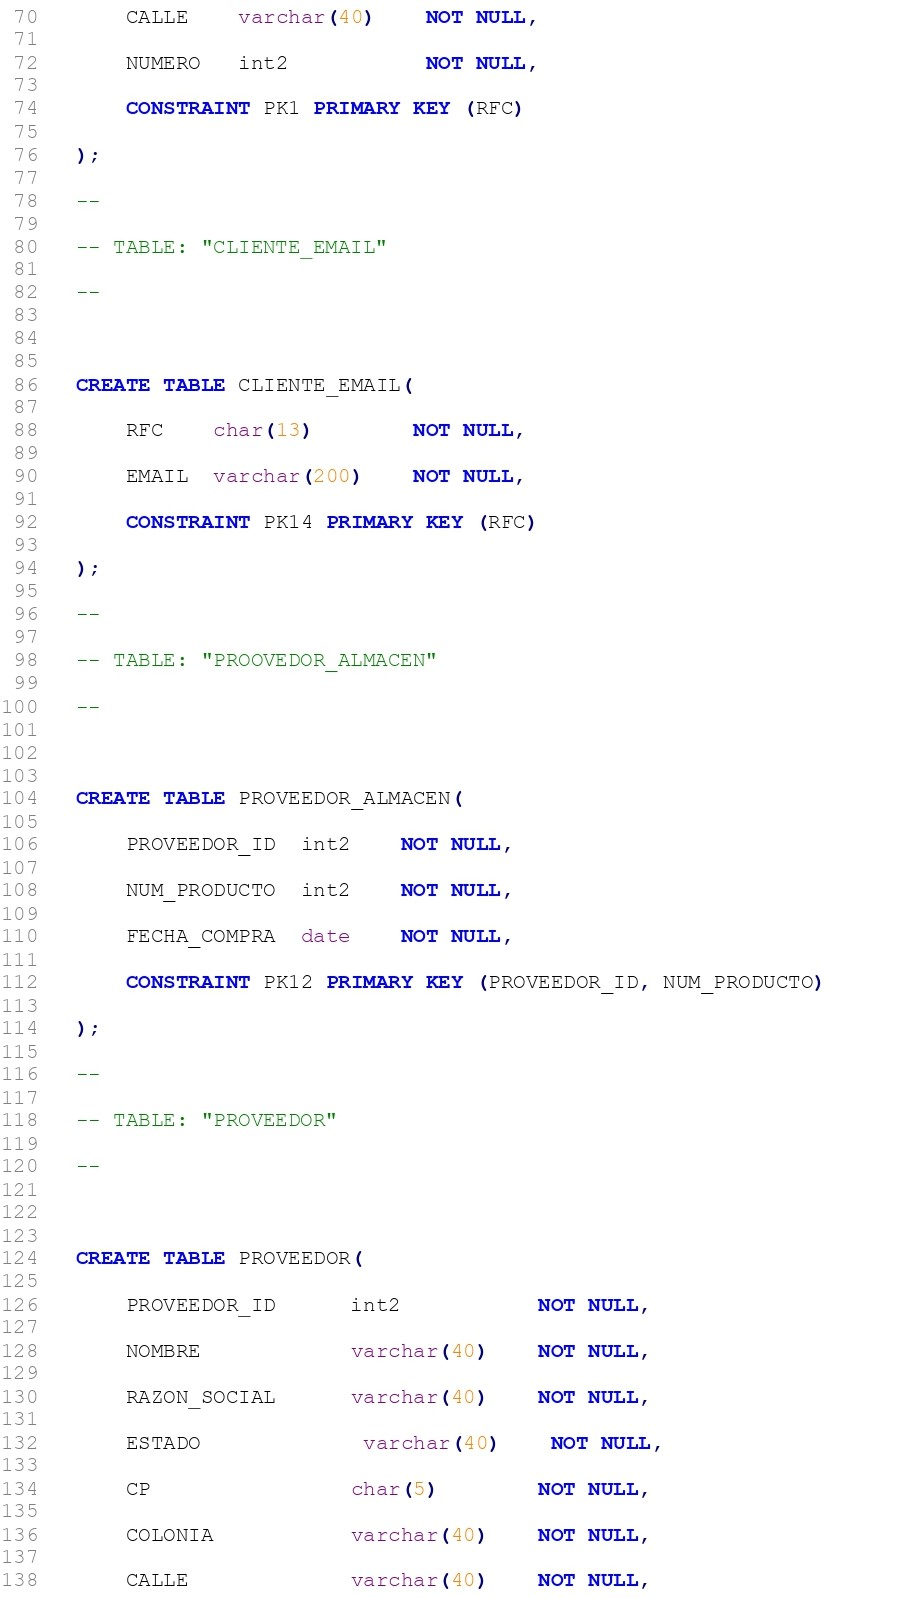
\includegraphics[scale=0.85]{imagenes/DDL2.jpg}
\newpage
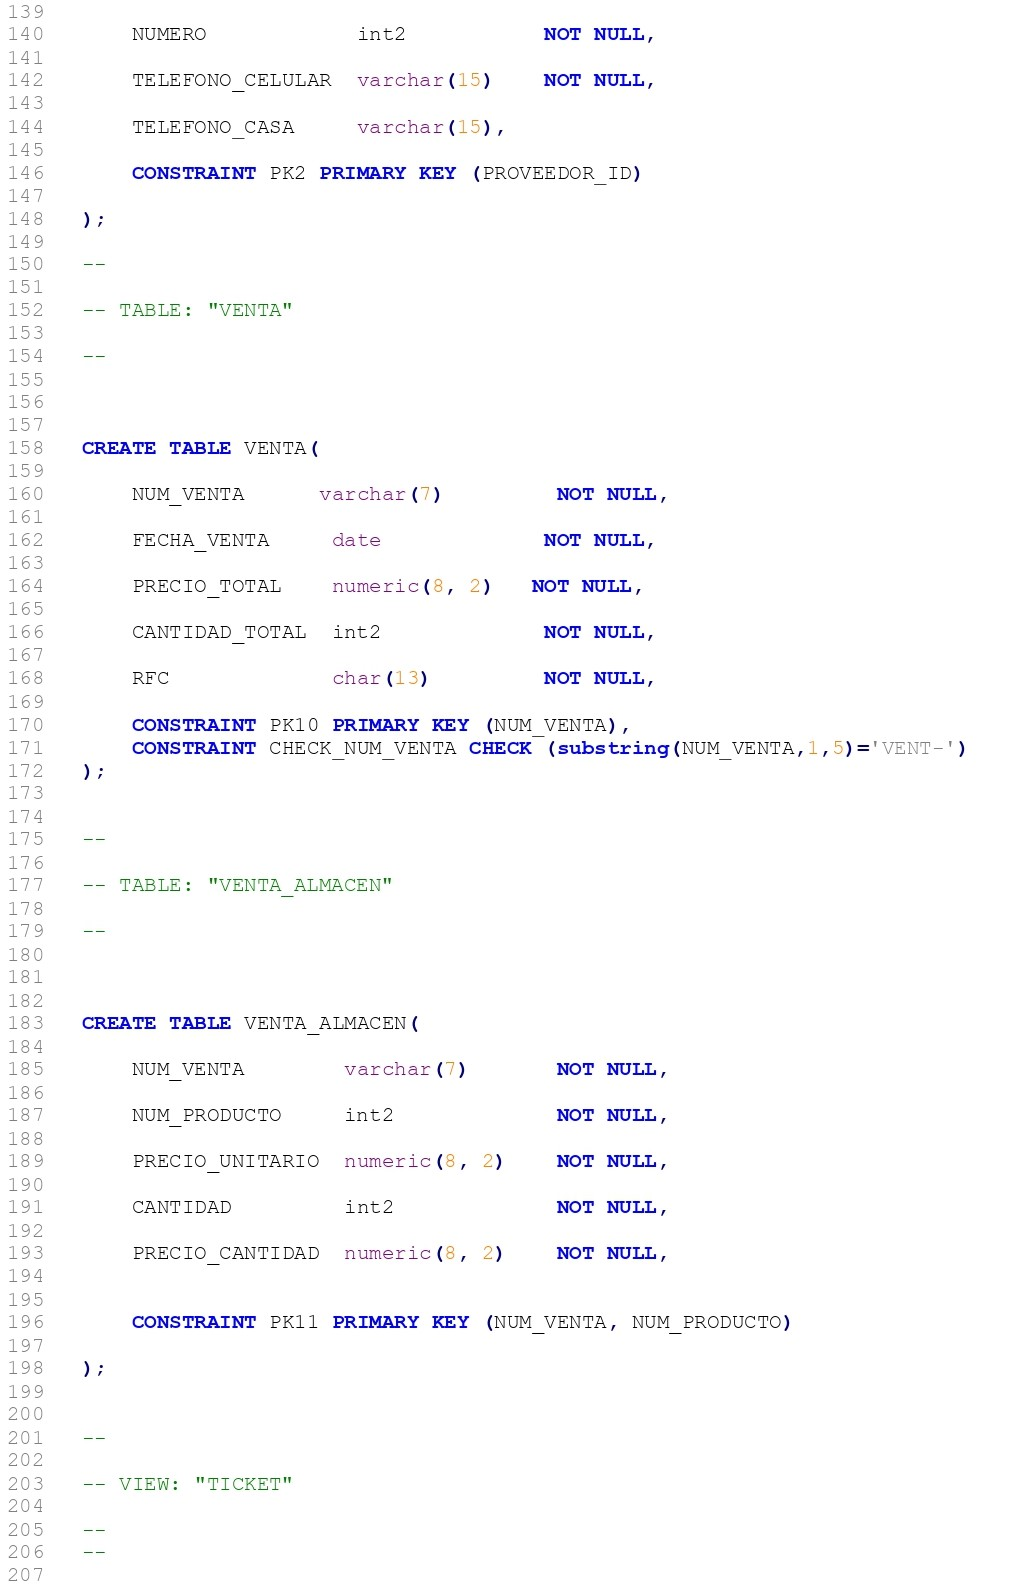
\includegraphics[scale=0.85]{imagenes/DDL3.jpg}
\newpage
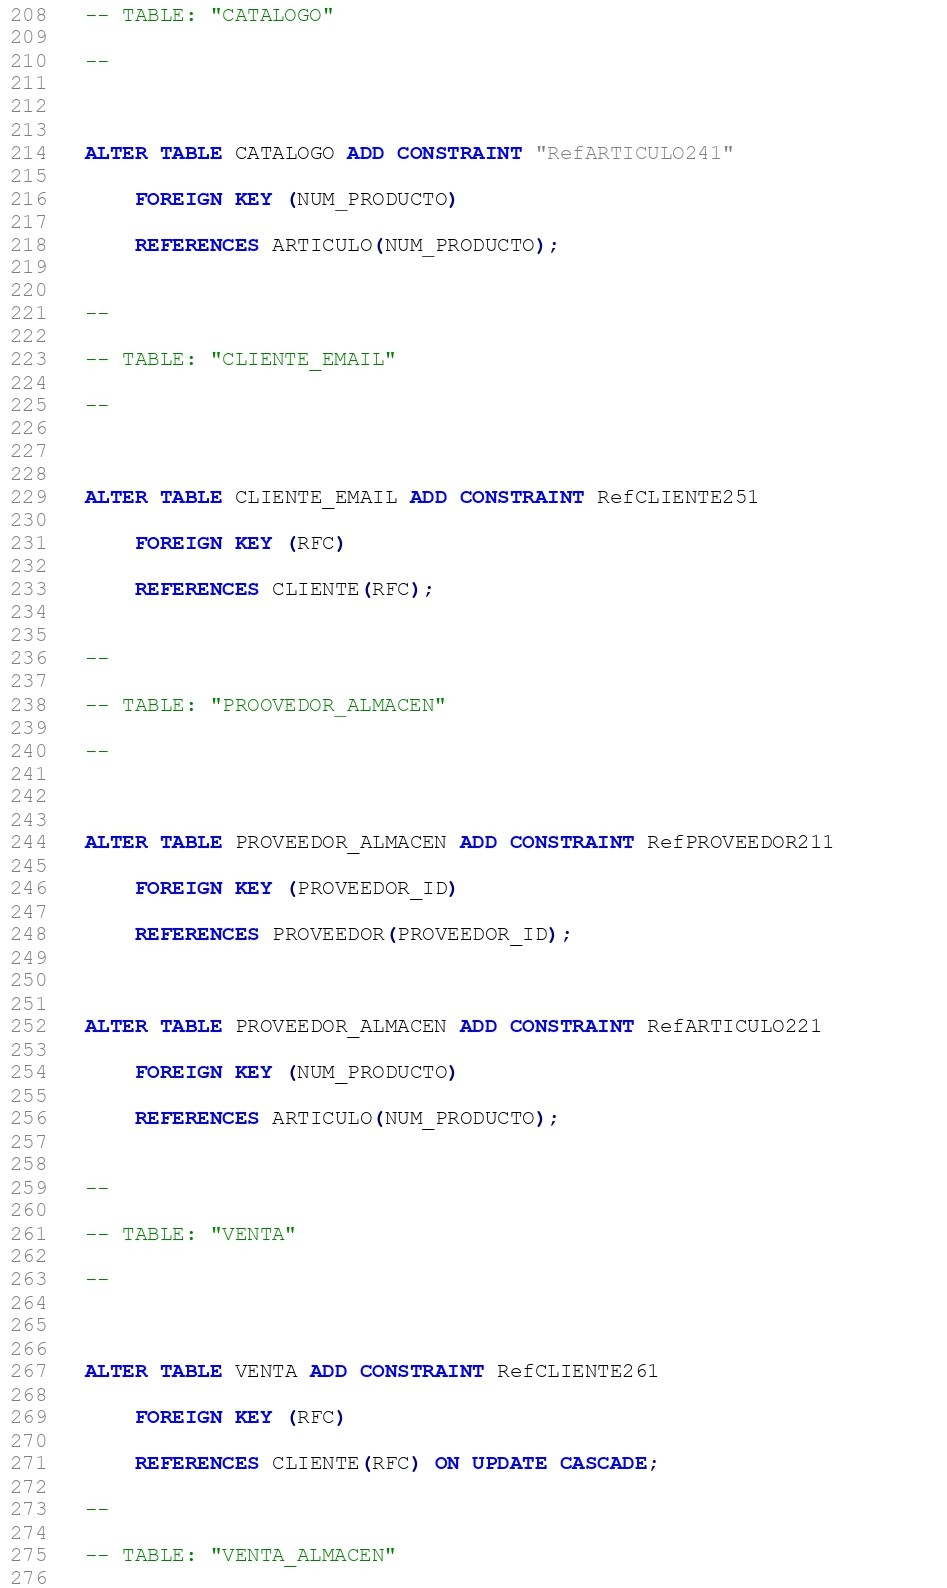
\includegraphics[scale=0.85]{imagenes/DDL4.jpg}
\newpage
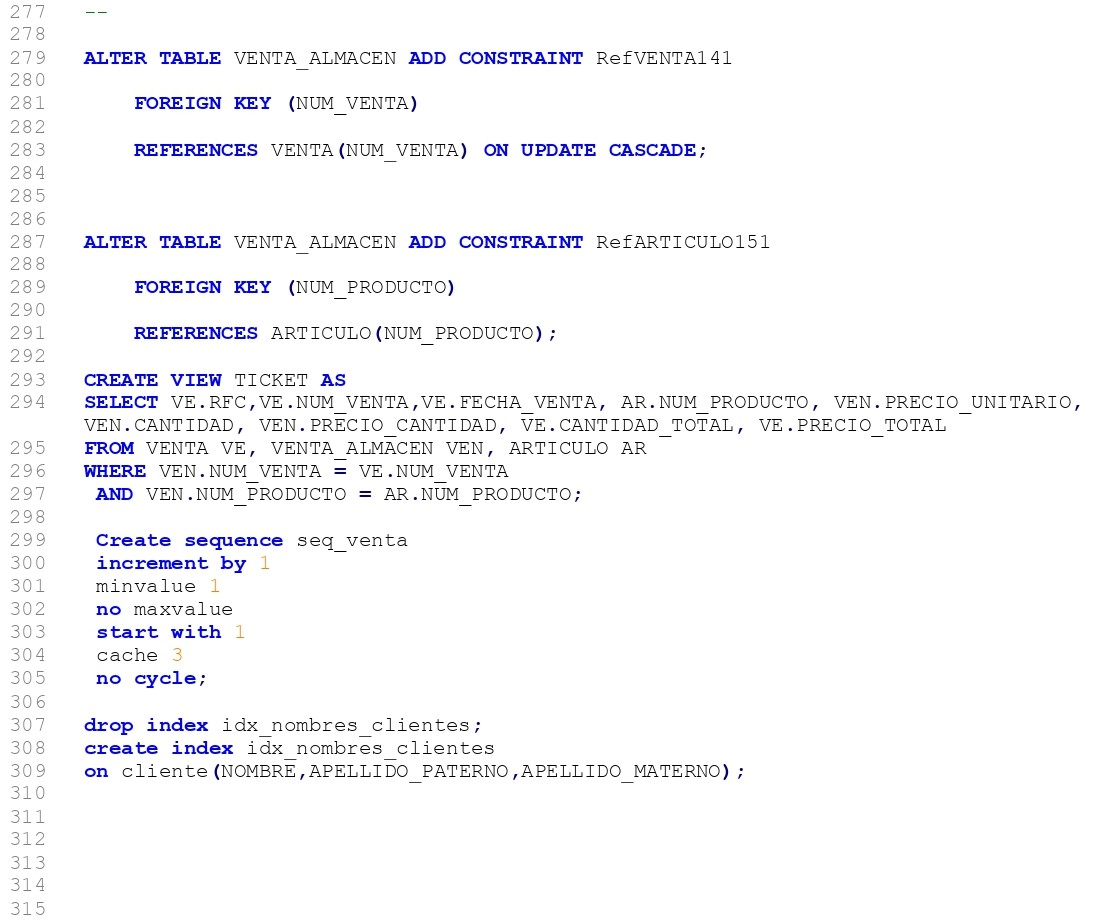
\includegraphics[scale=0.85]{imagenes/DDL5.jpg}
\newpage
Además se hizo una inserción de algunos registros para poderlos visualizar en la base de datos más adelante. El código SQL de los registros es el siguiente:
\\\\
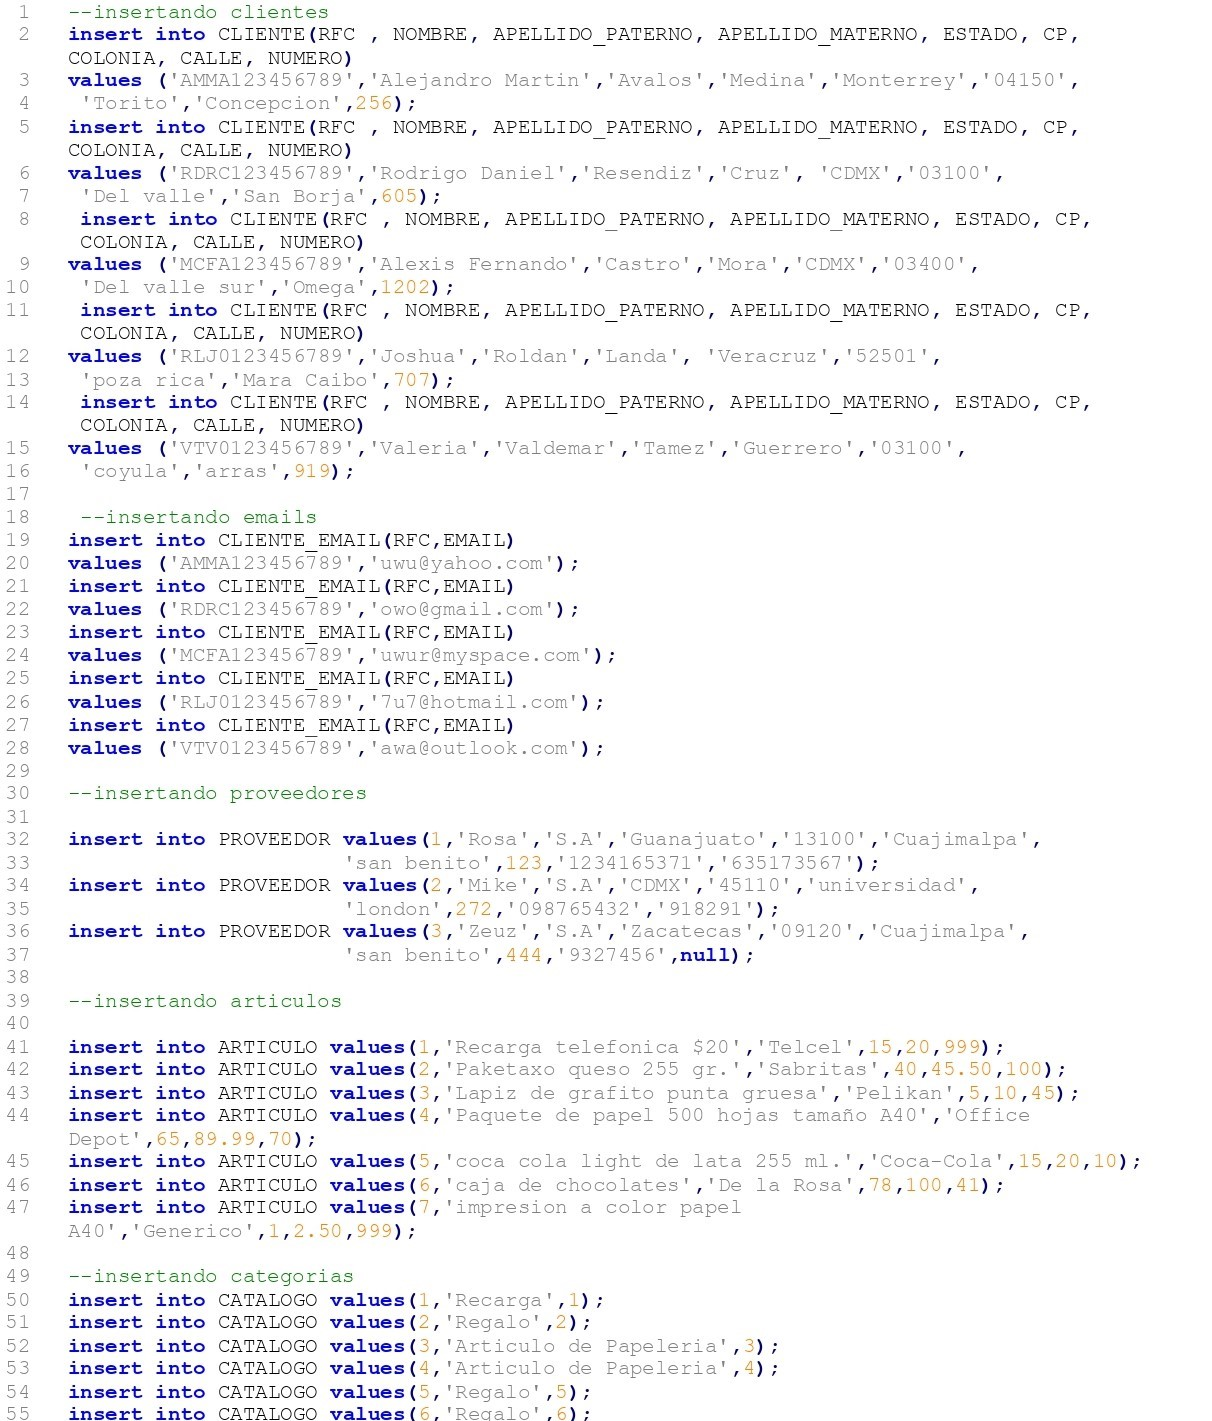
\includegraphics[scale=0.85]{imagenes/DML01.jpg}
\newpage
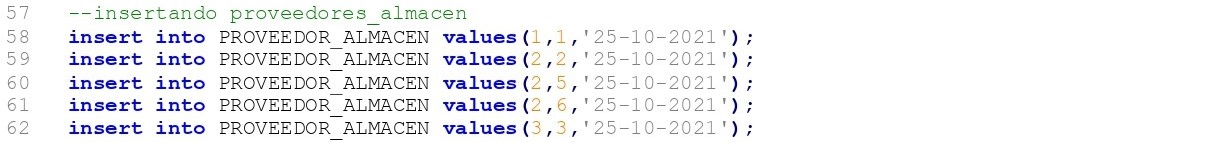
\includegraphics[scale=0.85]{imagenes/DML02-1.jpg}
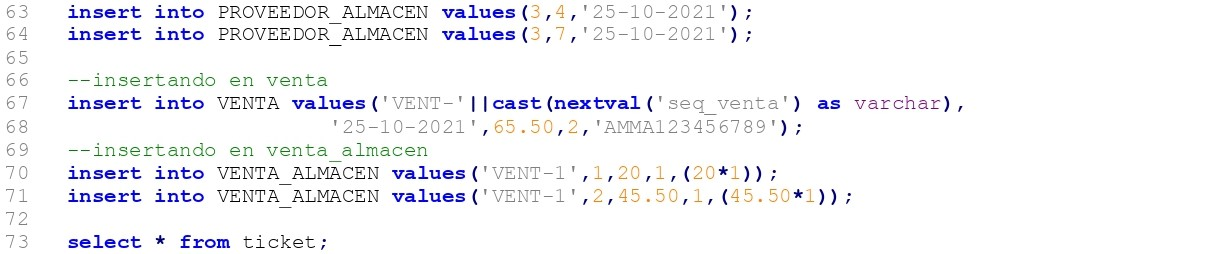
\includegraphics[scale=0.85]{imagenes/DML02-2.jpg}
\\\\\\
\large{ \textbf{Presentaci\'on}}
\\\\
Funcionamiento de la conexión de la base de datos a la interfaz gráfica:
\begin{enumerate}
\item Tener nuestra base de datos creada en nuestro manejador, en este caso con pgAdmin 4:
\begin{center} 
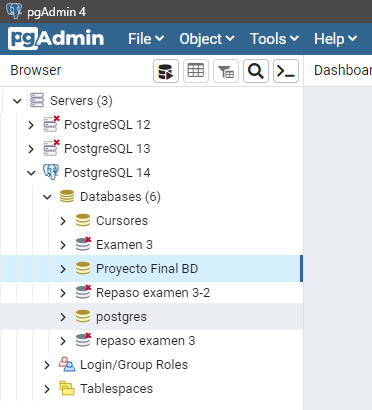
\includegraphics[scale=0.85]{imagenes/P01.png}
\end{center}
\newpage 
\item Tener o crear una cuenta con dominio educativo o empresarial en microsoft para acceder a una de sus aplicaciones, llamada Power Apps:
\begin{center} 
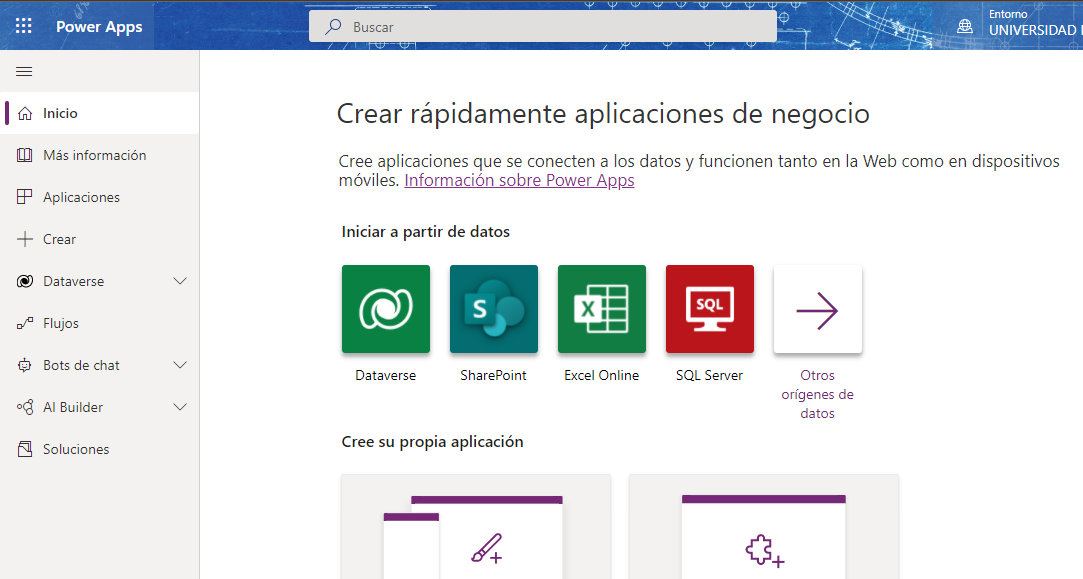
\includegraphics[scale=0.53]{imagenes/P02.png}
\end{center} 
\item Después le damos en crear y nos aparece la siguiente pantalla:
\begin{center} 
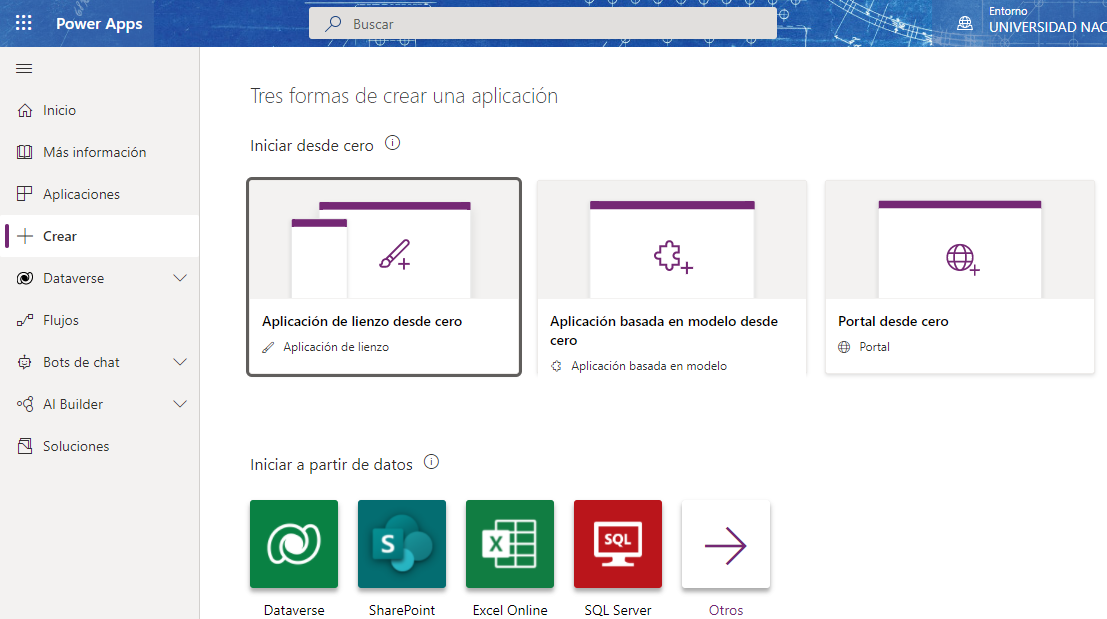
\includegraphics[scale=0.53]{imagenes/P03.png}
\end{center} 
\newpage
\item En la sección “Iniciar a partir de datos”, le damos clic en la flecha donde dice “Otros”  y nos parece la siguiente pantalla, donde elegiremos nueva conexión y buscaremos PostgreSQL como se muestra a continuación:
\begin{center} 
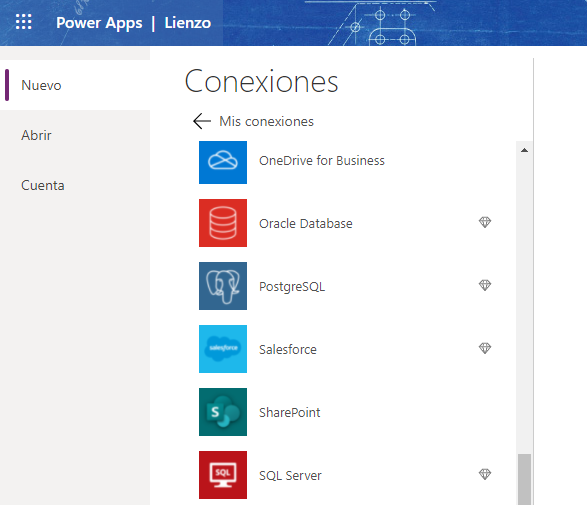
\includegraphics[scale=0.55]{imagenes/P04.png}
\end{center} 
\item Seleccionamos PostgreSQL, y buscamos al final del submenú, “Instalar puerta de enlace” cómo se ve a continuación:
\begin{center} 
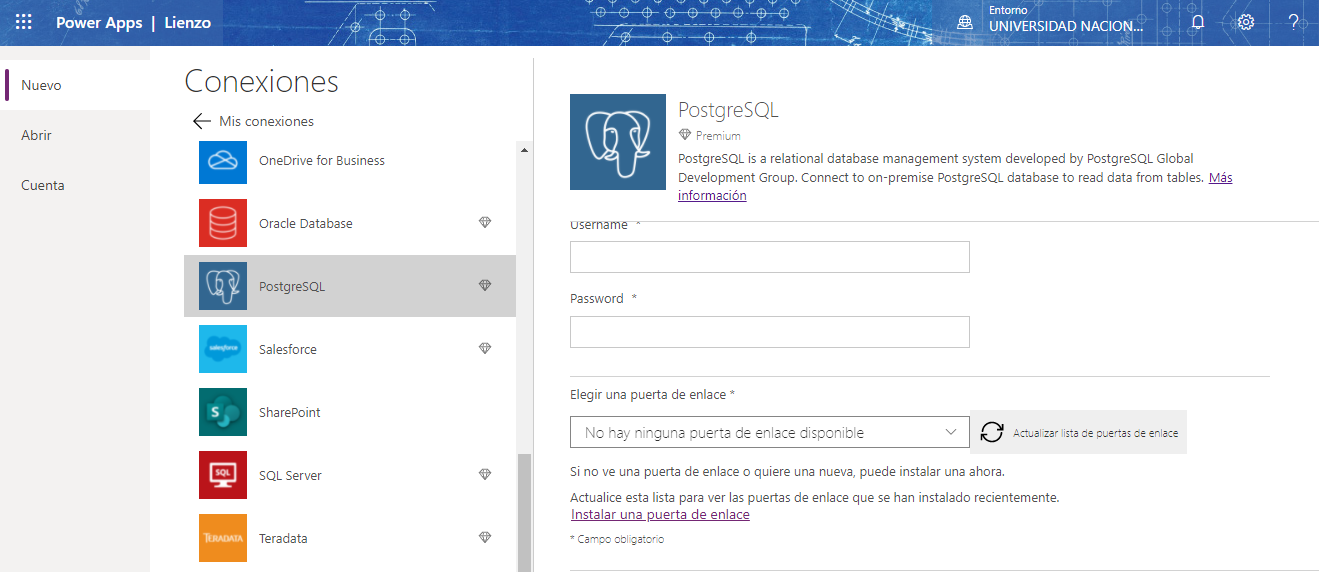
\includegraphics[scale=0.43]{imagenes/P05.png}
\end{center} 
\newpage
\item Después nos parece la siguiente pantalla, y le damos clic en “Puerta de enlace de datos on-premises” descargar:
\begin{center} 
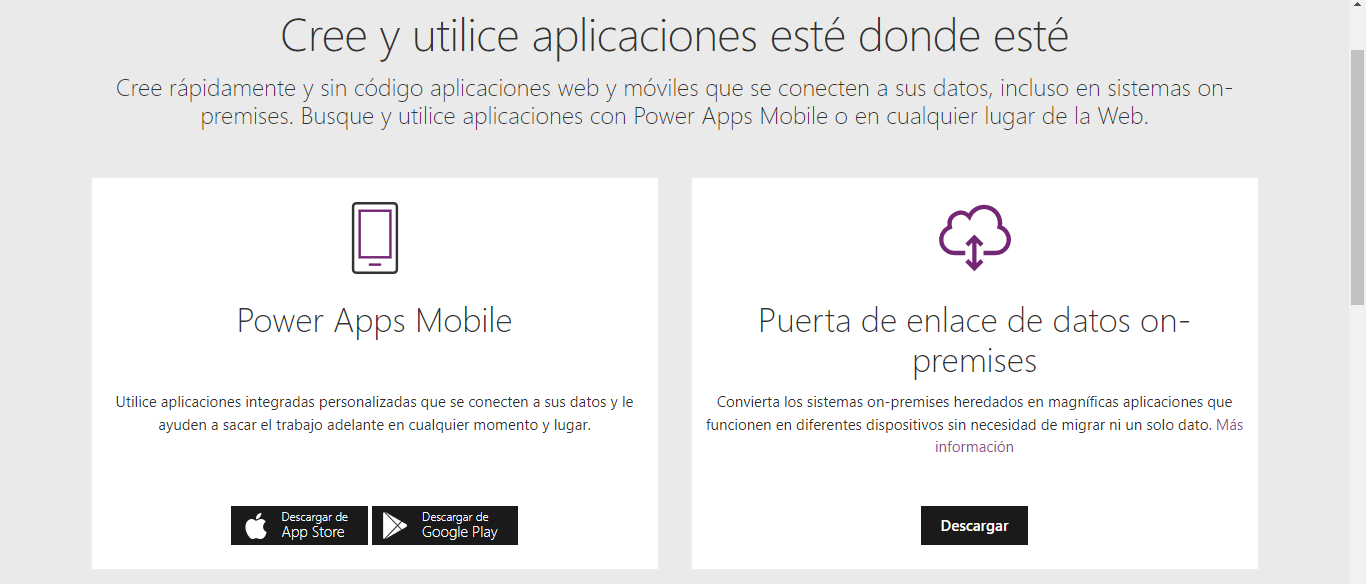
\includegraphics[scale=0.43]{imagenes/P06.png}
\end{center} 
\item Después aceptamos los permisos y empieza a instalar cómo se observa en la siguiente imagen:
\begin{center} 
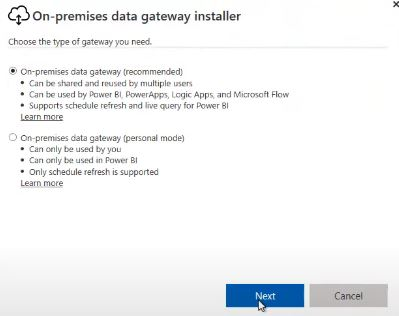
\includegraphics[scale=0.95]{imagenes/P07.jpg}
\end{center} 
\newpage
\item Luego nos pide el correo con el que iniciamos sesión en Power Apps, con el que enlazará, como se observa en la imagen:
\begin{center} 
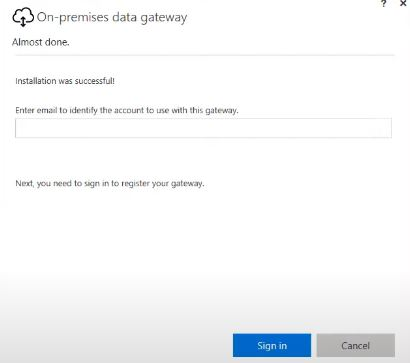
\includegraphics[scale=0.95]{imagenes/P08.jpg}
\end{center}
\item En el siguiente paso nos pide el nombre de data gateway y la contraseña, cómo se observa a continuación:
\begin{center} 
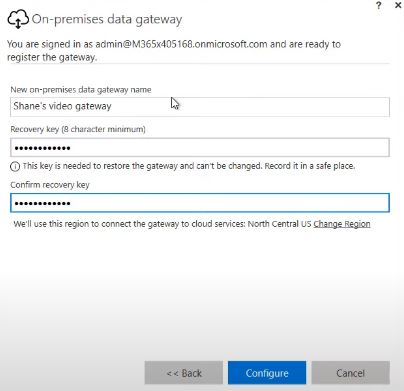
\includegraphics[scale=0.95]{imagenes/P09.jpg}
\end{center} 
\newpage
\item Después nos muestra el estatus del enlace con Power Apps, que fue exitoso:
\begin{center} 
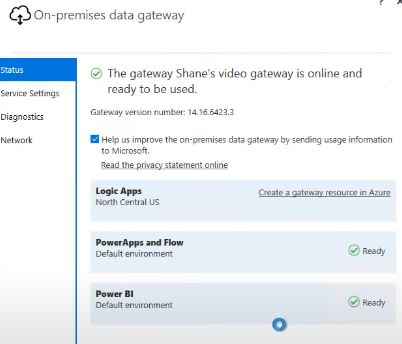
\includegraphics[scale=0.95]{imagenes/P10.jpg}
\end{center}
\item Por último nos regresa al formulario para llenar con los datos de nuestra base de datos creada con anterioridad en el manejador pgAdmin 4:
\begin{center} 
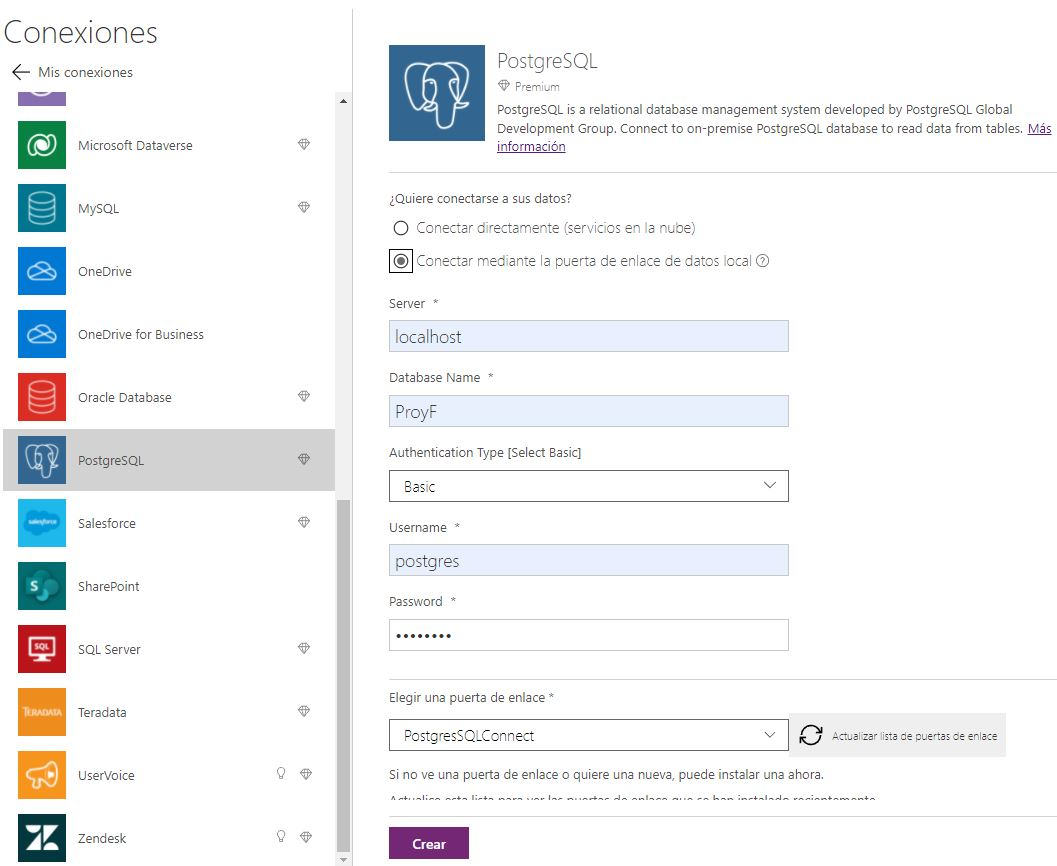
\includegraphics[scale=0.45]{imagenes/P11.jpg}
\end{center} 
\newpage
\item Una vez ya enlazada nuestra base de datos con Power apps, nos regresamos a la página de inicio y le damos en la primera opción “Aplicación de lienzo desde cero” y nos parece la siguiente pantalla:
\begin{center} 
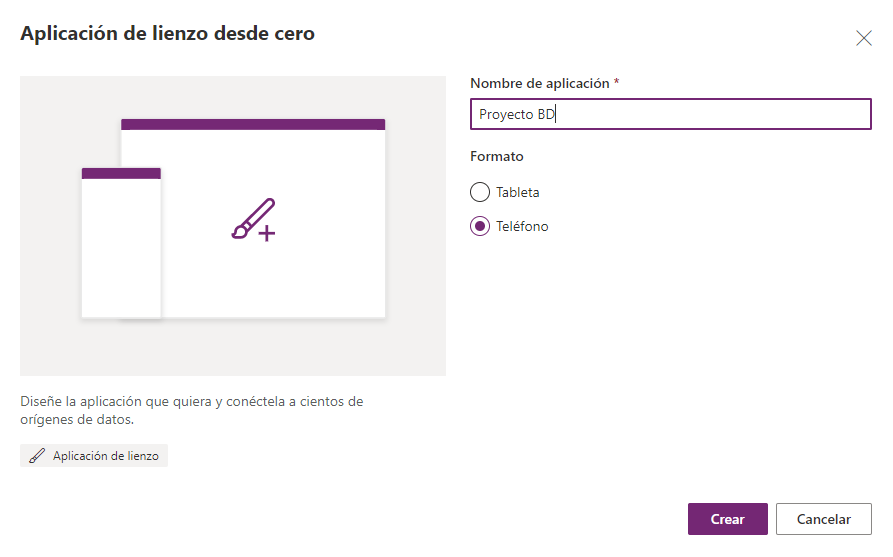
\includegraphics[scale=0.65]{imagenes/P12.png}
\end{center} 
Donde elegimos un nombre para nuestra aplicación, en nuestro caso Proyecto BD. Formato Teléfono, y le damos en crear.
\\
\item Nos direcciona a una nueva pantalla, donde nos permite diseñar y crear nuestra interfaz gráfica, una aplicación para smartphone, que es la siguiente:
\begin{center} 
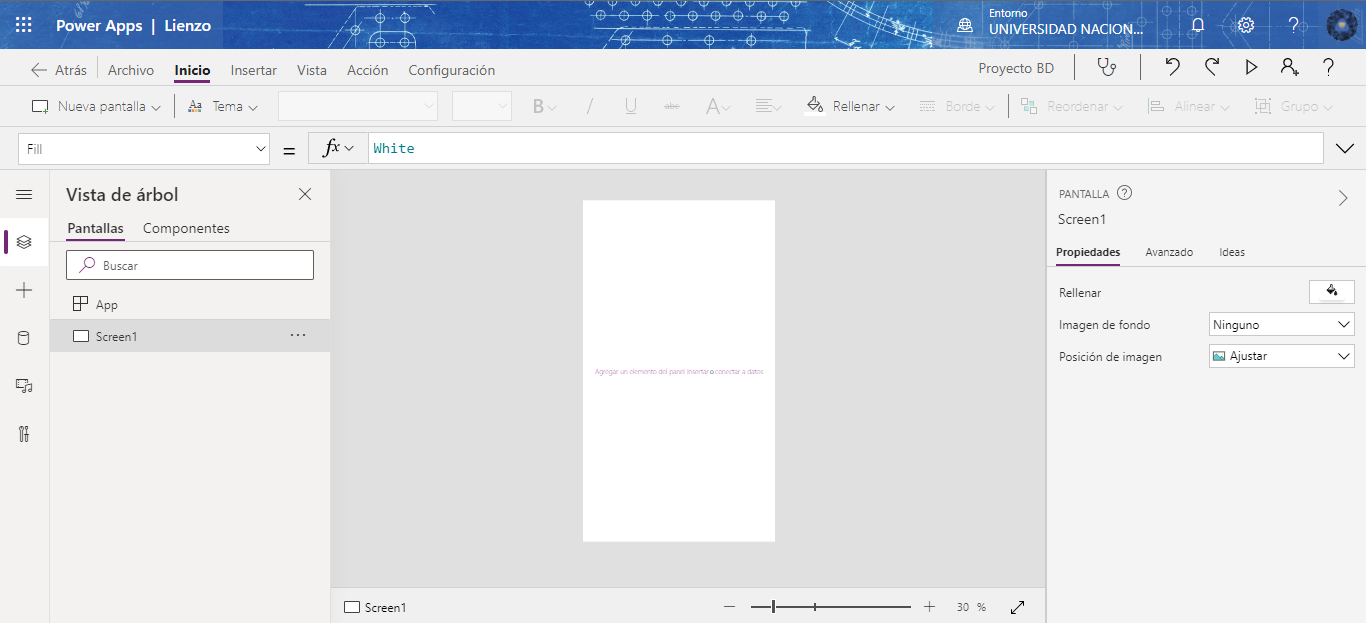
\includegraphics[scale=0.43]{imagenes/P13.png}
\end{center} 
\item Le damos clic en el símbolo de base de datos,buscamos la base de datos de PostgreSQL, en automatico Power Apps mostra la primer tabla que encuentre ya en una vista de la aplicación, como se ve a continuación:
\begin{center} 
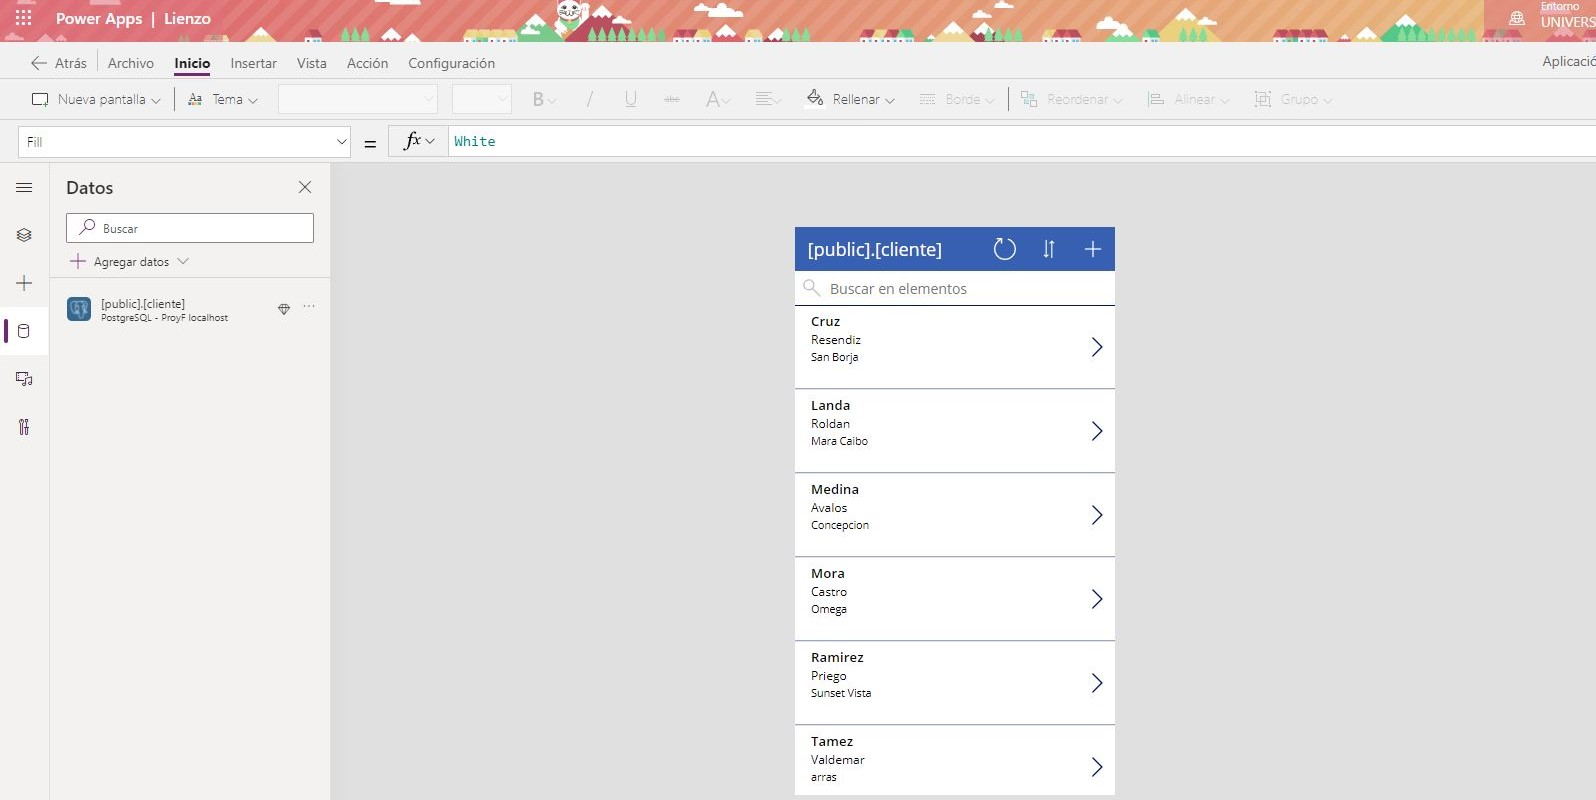
\includegraphics[scale=0.36]{imagenes/P14.jpg}
\end{center}
\item Por último podremos ver todas las tablas de nuestra base de datos, que podremos elegir para crear vistas o pantallas de nuestra aplicación, de acuerdo al diseño de la interfaz que queramos desarrollar, cómo observamos en la siguiente imagen:
\begin{center} 
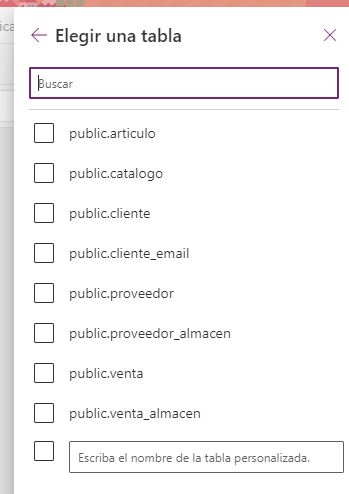
\includegraphics[scale=0.70]{imagenes/P15.jpg}
\end{center}
\end{enumerate}



\newpage 
Funcionamiento de la aplicación:
\begin{center} 
\includegraphics[scale=0.45]{imagenes/A01.jpeg}
\end{center}
La imagen que se muestra es la primera pantalla de la aplicación, aquí únicamente podemos observar el logo de papelería e interactuar con el botón para iniciar la aplicación.\\
\begin{center} 
\includegraphics[scale=0.45]{imagenes/A02.jpeg}
\end{center} 
Este es el menú principal de nuestra aplicación, como observamos, la etiqueta muestra automáticamente el nombre del usuario que esté haciendo uso de la aplicación, además de eso observamos un menú que se compone de tres opciones, de la cuál debemos elegir una.\\

\begin{center} 
\includegraphics[scale=0.45]{imagenes/A03.jpeg}
\end{center} 
Esta es la pantalla de nueva venta, aquí se muestra un listado de los productos que existen en inventario junto con algunas de sus características, el usuario debe seleccionar la cantidad del producto y marcar la casilla para que el elemento se agregue al carrito, incluímos una etiqueta que hace el conteo de los elementos en el carrito, también añadimos un botón para limpiar el carrito y un ícono para regresar al menú principal. Cuando el usuario termine de escoger los productos, debe presionar el ícono del carrito.\\
\begin{center} 
\includegraphics[scale=0.45]{imagenes/A04.jpeg}
\end{center} 
Al presionar el ícono del carrito de compras llegaremos a esta pantalla donde tendremos un resumen de la compra, observaremos una etiqueta que nos mostrará el total de la venta, posteriormente el usuario deberá ingresar el RFC y el correo electrónico de la persona a la que se desee enviar la orden de compra, al presionar el botón se enviará el correo y nos regresará al menú principal.\\

\begin{center} 
\includegraphics[scale=0.45]{imagenes/A05.jpeg}
\end{center} 
En el menú principal también podemos seleccionar la opción de inventario, la cual nos llevará a esta pantalla donde podremos ver la cantidad de artículos junto con sus características así como las de los proveedores, también nos podemos regresar al menú principal presionando el ícono del lado superior izquierdo.\\
\begin{center} 
\includegraphics[scale=0.45]{imagenes/A06.jpeg}
\end{center} 
La tercera opción del menú principal es la de clientes, al seleccionarla nos llevará a esta pantalla donde tendremos un listado de los clientes, desde aquí podremos actualizar la base de datos, ya sea modificando, eliminando o agregando un nuevo cliente, presionando la flecha que se encuentra del lado derecho de cada registro, podemos ver los detalles del cliente.\\

\begin{center} 
\includegraphics[scale=0.45]{imagenes/A07.jpeg}
\end{center} 
Esta pantalla es donde se muestran los detalles de los clientes, desde aquí podremos eliminar el registro o editarlo y cual sea la opción que escojamos se verá reflejada en nuestra base de datos.\\
\begin{center} 
\includegraphics[scale=0.45]{imagenes/A08.jpeg}
\end{center}
Este es el menú para editar un registro existente, podremos modificar cualquier campo y al terminar los cambios debemos presionar el ícono del lado superior derecho para confirmar los cambios.\\

\begin{center} 
\includegraphics[scale=0.45]{imagenes/A09.jpeg}
\end{center} 
Esta pantalla es para agregar a un nuevo cliente, tendremos que completar los campos y al finalizar confirmar la operación presionando el ícono del lado superior derecho, así mismo podremos cancelar la operación presionando el ícono de la X.\\\\\\
\large{ \textbf{Conclusiones}}
\\\\\textbf{\textit{Jimenez Avila Javier Alejandro}}
\\
La realización de este proyecto fue de suma importancia, ya que la problemática a resolver, se parece o es un problema de la vida real, lo cual nos generó trabajar y organizarnos cómo si fuéramos un equipo de desarrollo de una empresa. La organización de nuestros tiempos fue un punto clave para el buen desarrollo y avance del proyecto, realizamos reuniones por la plataforma meet para; revisar entregas internas, problemáticas emergentes, soluciones, y revisión de todo aquello que se hacía o faltaba. Se puso en práctica todo lo que vimos en el curso, como fue el diseño de una base de datos, por medio del desarrollo de modelos (MER, MR), la creación de tablas, llaves, consultas, operaciones en las tablas, funciones y procedimientos de una base de datos, entre otros conocimientos vistos en el curso. Además aprendimos nuevas herramientas, cómo fue la implementación de una interfaz gráfica, que de primera instancia, se nos dificulto un poco, pero encontramos una solución sutil, por medio de Power Apps. Considero que este proyecto explotó todos los conocimientos adquiridos durante el curso, lo que reforzó y estímulo a aprender otros. Esto se vuelve una herramienta útil y de mucha importancia para nuestra formación académica.
\\\\\textbf{\textit{Mora Castro Fernando Alexis}}
\\
Considero que este proyecto fue un verdadero reto, sin embargo, fue muy satisfactorio ver el resultado final. Llegar al resultado final involucró aplicar todos los conocimientos vistos en clase e incluso indagar un poco más acerca de temas que no conocíamos por ejemplo como hacer la conexión de la base de datos con la interfaz gráfica, como logro personal me agradó que tuve la oportunidad de aplicar conocimientos que adquirí en mi trabajo actual, pero lo más importante fue el trabajo en equipo ya que nos ayudamos mutuamente y complementamos ideas en todo momento, en conjunto pudimos elaborar desde el modelo relacional hasta la interfaz gráfica.
\\\\\textbf{\textit{Resendiz Cruz Rodrigo Daniel}}
\\
En este proyecto vimos todo lo que involucra hacer una base de datos desde cero, comenzando por el planteamiento de una necesidad a resolver, pasando por el diseño de la solución a manera de base de datos, la identificación de la información a guardar, la generación de las tablas y la generación de registros que ilustran el guardado de la información y terminamos con la programación de excepciones que pueden presentarse en la base de datos los cuales se representan con los trigger. \\
Al final pudimos ser capaces de implementar una aplicación que nos permitiera ingresar información a la base de datos.
A lo largo de la realización de la base de datos logré identificar varios aciertos y errores en cuanto a nuestro desempeño, en cuanto a los aciertos puedo decir que en lo que estuvimos trabajando en el proyecto se mantuvo una buena comunicación ya que se organizaban juntas por medio de meet para tratar ciertos puntos importantes, por lo que, este tipo de comunicación dinámica nos ayudó a poder delimitar el problema y atacar ciertos puntos que no podiamos visualizar a simple vista. Por otro lado se nos dificultó iniciar con la implementación de la aplicación web ya que requería de cierto conocimiento que no teníamos, por esto mismo se tuvieron contratiempos inesperados y terminamos por optar usar la plataforma de aplicaciones power apps de microsoft para facilitar dicho desarrollo. Finalmente cabe mencionar que considero que este tipo de proyectos son el tipo de actividades que nos ayudan a poner a prueba el curso completo ya que necesitamos de cada conocimiento adquirido a través de éste para lograrlo realizar, espero que este curso nos traiga cosas buenas a futuro ya sea si decidimos a dedicarnos a la materia o decidimos usarla como herramienta complementaria a algo a lo que nos queremos especializar.
\\\\\textbf{\textit{Valdelamar Tamez Valeria}}
\\
En este proyecto pudimos aprender sobre cómo realizar una base de datos para la administración de una cadena de papelerías, se realizaron procedimientos que vimos en clase y aprendimos en ella desarrollando y poniendo en práctica nuestra habilidad para programas en el lenguaje Postgres.\\
Finalmente se realizaron diferentes tipos de consultas para poder cumplir con los requerimientos de la base en donde podemos observar diferentes procedimientos con triggers donde podemos observar la cantidad vendida por artículo, la cantidad total que se vendió y la garantía correspondiente a la fecha, obtener el nombre de los productos de los cuales hay menos de 3 en stock así como generar una vista en la cual se tiene la información necesaria para asemejarse a una factura.


		






\end{document}